\section{Present CSC Trigger Algorithm}
\label{sec:present_algo}

\subsection{ALCT Processing}

In the CSC muon system, anode wires are hardwired together at the readout end in groups of 10-15 wires in order to reduce channel count. The anode wire group signals are fed into the AFEB boards, each of which contains a single 16-channel amplifier/constant-fraction discriminator chip. The output signals from the AFEB boards are sent into the ALCT boards, which handle triggering and readout of CSC anode information. Due to the various types of CSC chambers, there are 3 sizes of ALCT boards, handling 288, 384, and 672 anode wire group channels.

On the ALCT boards, the signals from each AFEB are first delayed by a programmable amount in order to perform an average time alignment of the anode signals across the chamber as well as chamber-to-chamber at a sub-bunch crossing level to about 2.2 ns precision. After the AFEB signals are received and time-aligned, they are then latched with the bunch crossing frequency and fed to a Xilinx Virtex FPGA mounted on a mezzanine card above the ALCT main board for pattern-finding and readout functions.

The algorithm used in the Virtex FPGA of the ALCT for determining muon segment position and bunch crossing in the anode view is illustrated below. Since the drift time can be longer than 50 ns, the hits are first stretched by 'one-shots' to 6 bunch crossings (150 ns) length. Then, a multi-layer coincidence technique in the anode LCT pattern circuitry is used to identify the bunch crossing. For each spatial pattern of anode hits, a low coincidence level, typically 2 or more layers, is used to establish timing, whereas a higher coincidence level, typically 4 layers, is used to establish the existence of a muon track. The general idea of a spatial pattern of CSC wire group hits is illustrated below in Fig.\ref{fig:anode_wire_group_hits}.

\begin{figure}[tbh]
        \begin{center}
                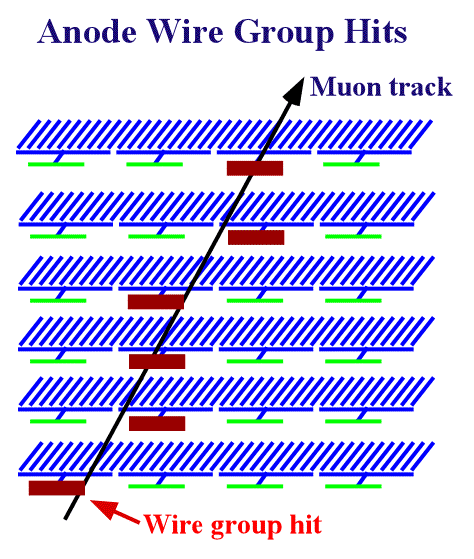
\includegraphics[width=0.48\linewidth]{figures/anode_wire_group_hits.png}
                \caption{CSC wire group patterns}
                \label{fig:anode_wire_group_hits}
        \end{center}
\end{figure}

while the general idea of the time stretching of hits, and pretrigger followed by a pattern trigger is shown in Fig.\ref{fig:anode_stretched_hits} (using an example in which one hit is actually missing due to some type of inefficiency).

\begin{figure}[tbh]
        \begin{center}
                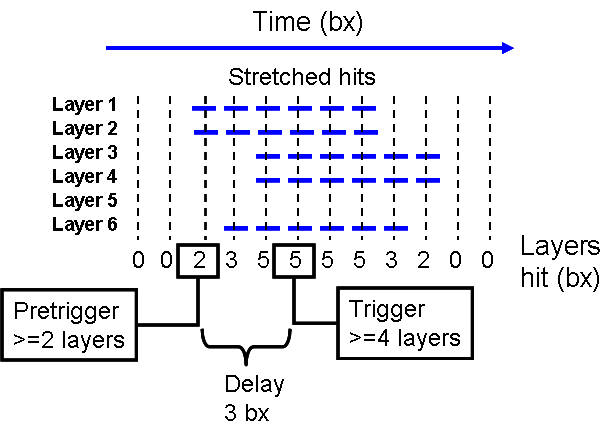
\includegraphics[width=0.73\linewidth]{figures/anode_stretched_hits.png}
                \caption{Anode stretched hits}
                \label{fig:anode_stretched_hits}
        \end{center}
\end{figure}

Each pattern detector can detect a programmable "collision" pattern as well as a fixed "accelerator" pattern. The input data for the collision pattern detector are selected as shown below:

\begin{center}
\begin{verbatim}
...n-2 n-1 n...........Layer 1
.......n-1 n...........Layer 2
...........n...........Layer 3
...........n n+1.......Layer 4
...........n n+1 n+2...Layer 5
...........n n+1 n+2...Layer 6
\end{verbatim}
\end{center}

where n in this diagram is the key wire group number, which this particular pattern detector is searching the patterns for. The programming of the programmable collision pattern is implemented as a simple masking-out of the bits that we do not want to include in the pattern. The accelerator pattern is a vertical pattern of 6 layers all with strip n only.

Each ALCT candidate is assigned a quality equal to number of layers with hits minus 3 and passes through a ghost cancellation procedure: it is cancelled if there is another ALCT candidate at the same bunch crossing in the previous wirewith the same or better quality or in the next wire with better quality, or if there is ALCT candidate up to 4 bunch crossing clocks earlier with any quality.

In each bunch crossing two ALCTs with highest quality are sent to the TMB (Trigger MotherBoard), which requires a coincidence between anode and cathode trigger information. In the case of a Level-1 Accept signal from the Global Trigger (distributed via the TTC system to the CCB in each peripheral crate), ALCT data are sequentially transmitted to the Trigger Mother Board and hence to the DAQ Motherboard. These data frames include a few words of ALCT trigger data and a much larger amount of ALCT raw hit data consisting of a time sequence of raw CSC anode wire-group hits that have been stored at the 40 MHz bunch crossing frequence by the ALCT2001. Typically 8 to 16 bunch crossings are read out for each wire group. FIFO data can also be read out much more slowly through VME access via the TMB board using a JTAG electrical interface to the ALCT, if necessary.

For self-monitoring and also for powering and controlling the AFEB cards, the ALCT contains a Slow Control section that supplies power to the AFEBs, controls AFEB thresholds, provides and controls the amplitude of test pulses to the AFEBs, and reads back power supply voltages and currents, as well as on-board temperature. 

\newpage
\subsection{Software Emulation of ALCT Processing}

ALCT processing includes the following five steps:

\begin{itemize}
    \item Pulse extension;
    \item Pretrigger;
    \item Trigger;
    \item Ghost cancellation;
    \item ALCT construction.
\end{itemize}

\subsubsection{Pulse Extension}

Sofware emulation provides information about all wire signals in DAQ readout window (16 BXs). A search for these signals is performed in a loop over all wire groups, all layers, and all 16 BXs; found signals are stretched over 6 BXs (see Fig.~\ref{fig:alct_pulse_extension}).

\begin{figure}[tbh]
        \begin{center}
                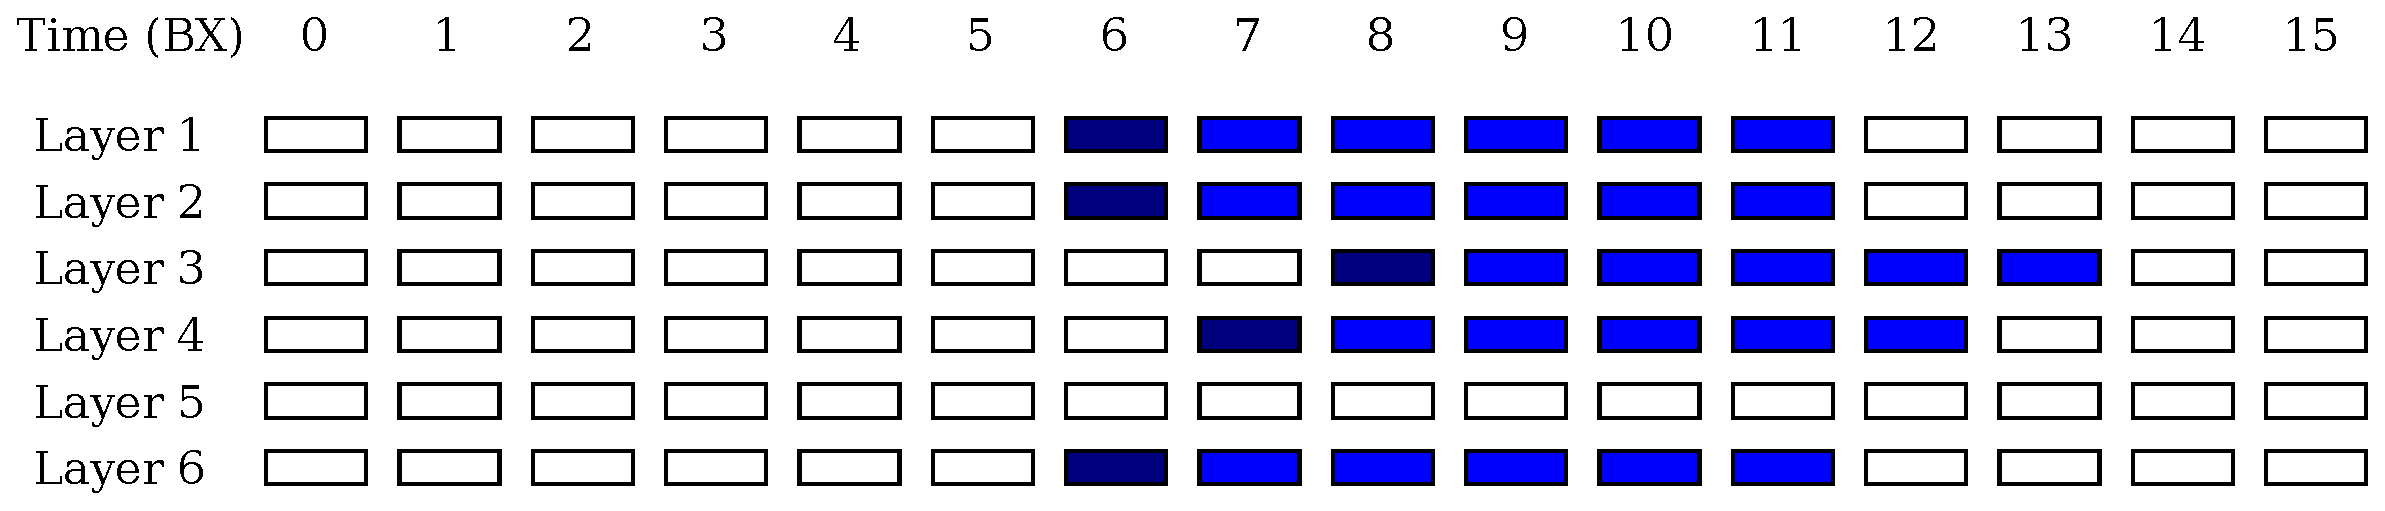
\includegraphics[width=0.9\linewidth]{figures/stretched_hits_alct.pdf}
                \caption{Illustration of ALCT pulse extension for one specific wire group.}
                \label{fig:alct_pulse_extension}
        \end{center}
\end{figure}

\subsubsection{Pretrigger}

After all available wire signals are stretched, a search for ALCT pretriggers is performed in all wire groups and all BXs. For any given wire group and BX, we count the number of layers with hits within the pattern mask shown on Fig.~\ref{fig:alct_pretrigger}, and if this number is greater than or equal to three, then we say that a pretrigger occured in this wire group and BX. The search for next ALCT pretrigger starts 6 BXs later.

\begin{figure}[tbh]
        \begin{center}
                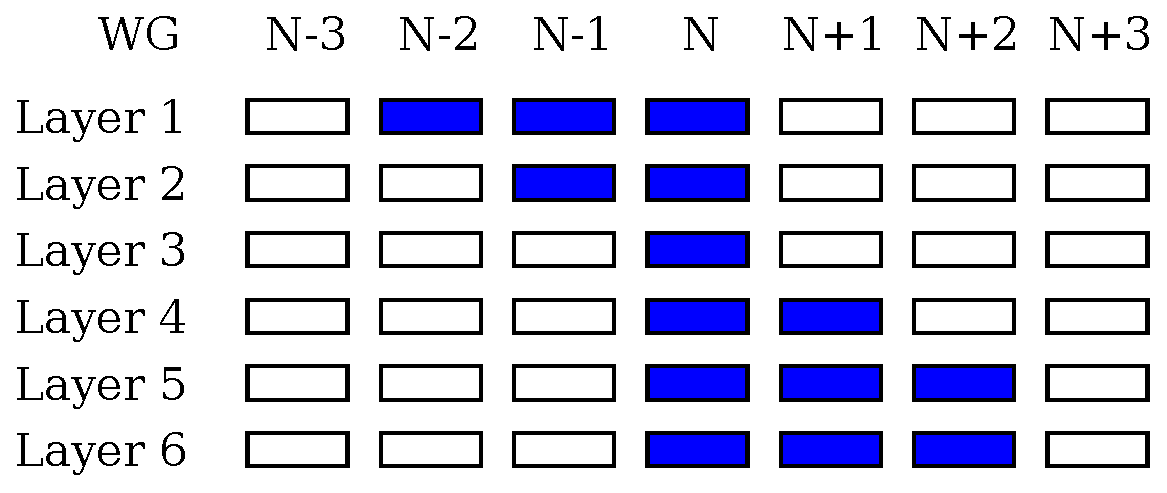
\includegraphics[width=0.45\linewidth]{figures/alct_pretrigger.pdf}
                \caption{ALCT pattern mask for pretriggering and triggering.}
                \label{fig:alct_pretrigger}
        \end{center}
\end{figure}

\subsubsection{Trigger}

After all ALCT pretriggers are found, for each pretrigger in BX = B we check for a trigger in BX = B+2. For any given wire group and BX = B+2, we count the number of layers with hits within the same pattern mask used for pretriggering, and if this number is greater than or equal to four, we say that a pretrigger occured in this wire group and BX, and assign it a quality Q = number of layers with hits-3. If in some wire group more than one trigger occured, we report only the one with the highest quality. If there are two triggers with the same quality, report the earlier one.

\subsubsection{Ghost Cancellation}

Not all triggers found in the previous step are used to construct ALCTs: before that all of them pass through so called ghost cancellation procedure.

A trigger in wire group = N and BX = B is cancelled if there is a trigger in wire group = N-1:
\begin{itemize}
    \item either in the same BX = B and with better or equal quality;
    \item or to 4 BXs earlier, with any quality.
\end{itemize}

In addition, a trigger in wire group = N and BX = B is cancelled if there is a trigger in wire group = N+1:
\begin{itemize}
    \item either in the same BX = B and with better quality;
    \item or to 4 BXs earlier, with any quality.
\end{itemize}

\subsubsection{ALCT Construction}

Construct ALCTs from triggers survived after the ghost cancellation procedure: encode quality, WG, BX (defined by pretrigger BX). In every BX choose best two ALCTs: two ALCTs with the highest quality. If we need to choose one ALCT from two ALCTs with the same quality: choose the one with larger wire group.

\newpage
\subsection{CLCT Processing}

[We need a good picture illustrating CLCT processing process like in the case of ALCT one]

A muon passing through a CSC chamber will produce distinctive patterns of half-strip
hits in the six-layer endcap muon CSC chambers. By identifying these patterns, the CSC Local
Trigger provides high rejection power against backgrounds. The largest background source,
neutron-induced gamma ray conversions, are generally low in energy, and produce mostly single-
layer or short multi-layer hits. Other backgrounds, such as low-momentum muons or punch-
through particles often do not point well enough to the primary interaction region to be considered
high-momentum muon candidates.

\begin{figure}[tbh]
        \begin{center}
                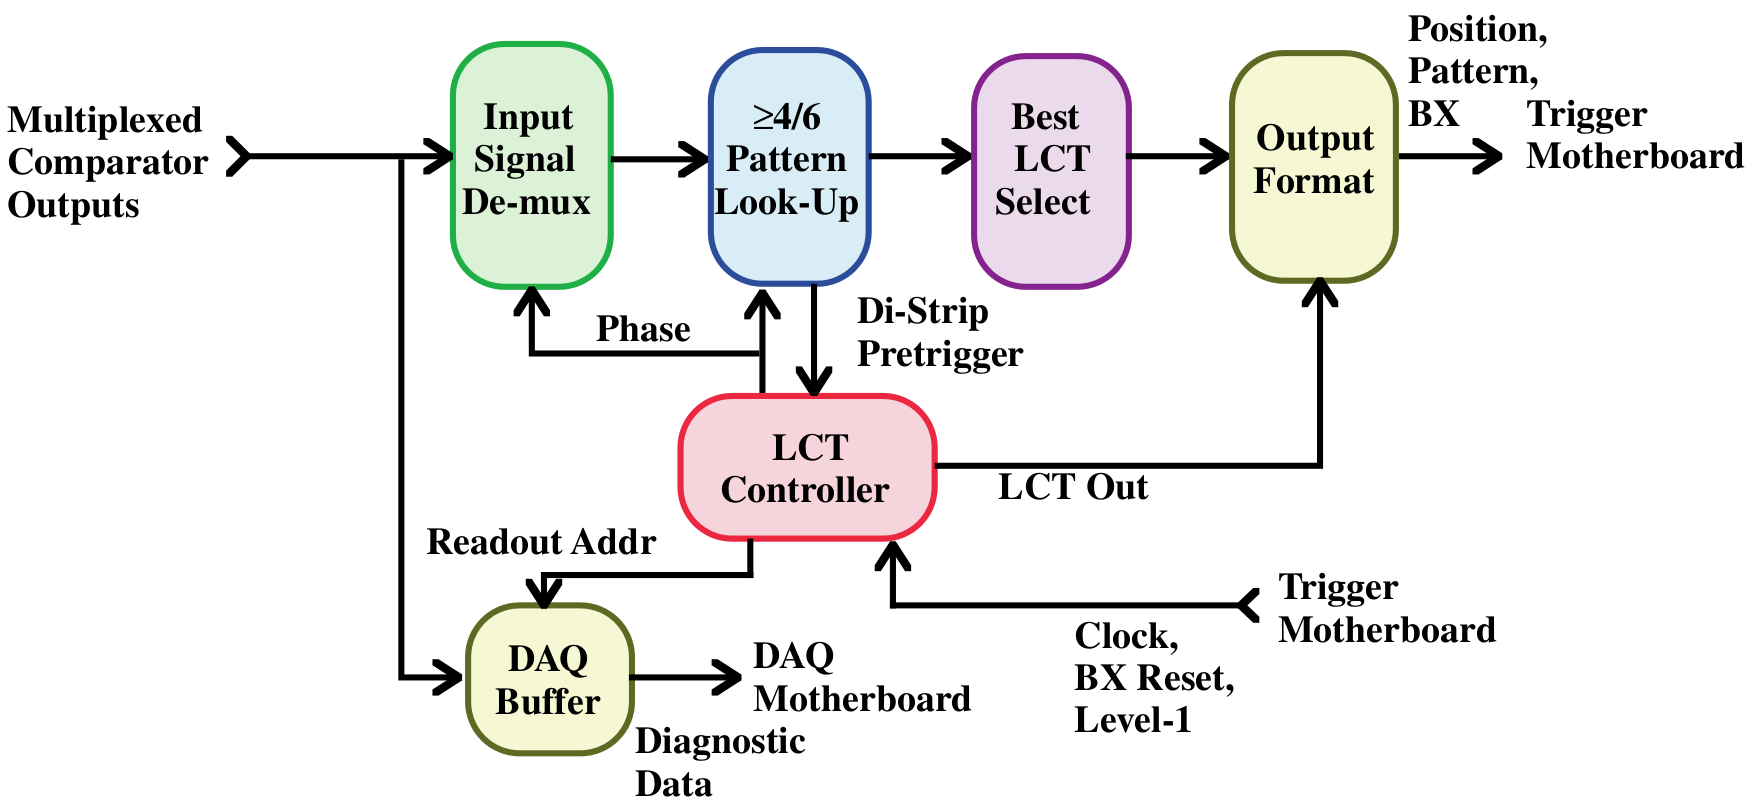
\includegraphics[width=0.73\linewidth]{figures/CLCT_block_diagram.png}
                \caption{CLCT block diagram}
                \label{fig:clct_block_diagram}
        \end{center}
\end{figure}

[Technical description from TMB manual below]

For each of 160 key half-strips consider the 42 neighboring half-strips (i.e. on key 5 use the following half-strips):

\begin{figure}[tbh]
        \begin{center}
                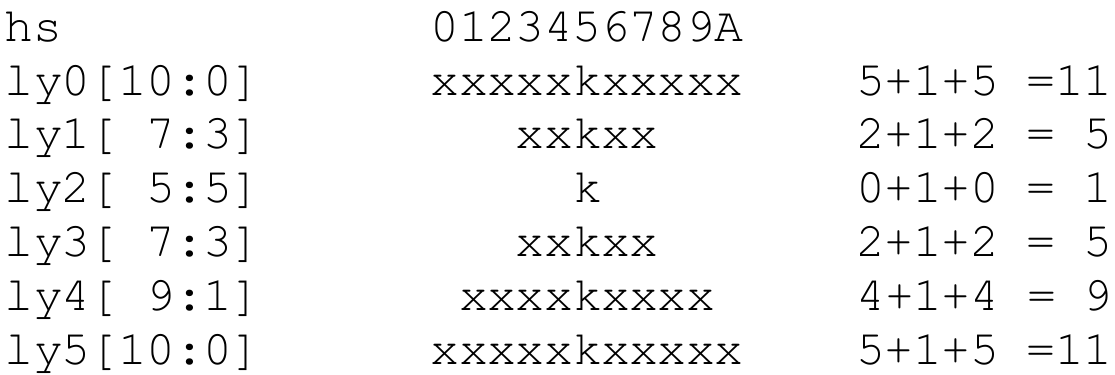
\includegraphics[width=0.48\linewidth]{figures/160_key_half_strips.png}
                \caption{160 key half-strips}
                \label{fig:160_key_half_strips}
        \end{center}
\end{figure}

For each of 160 key half-strips, count layers with hits matching the 9 pattern templates:

\begin{figure}[tbh]
        \begin{center}
                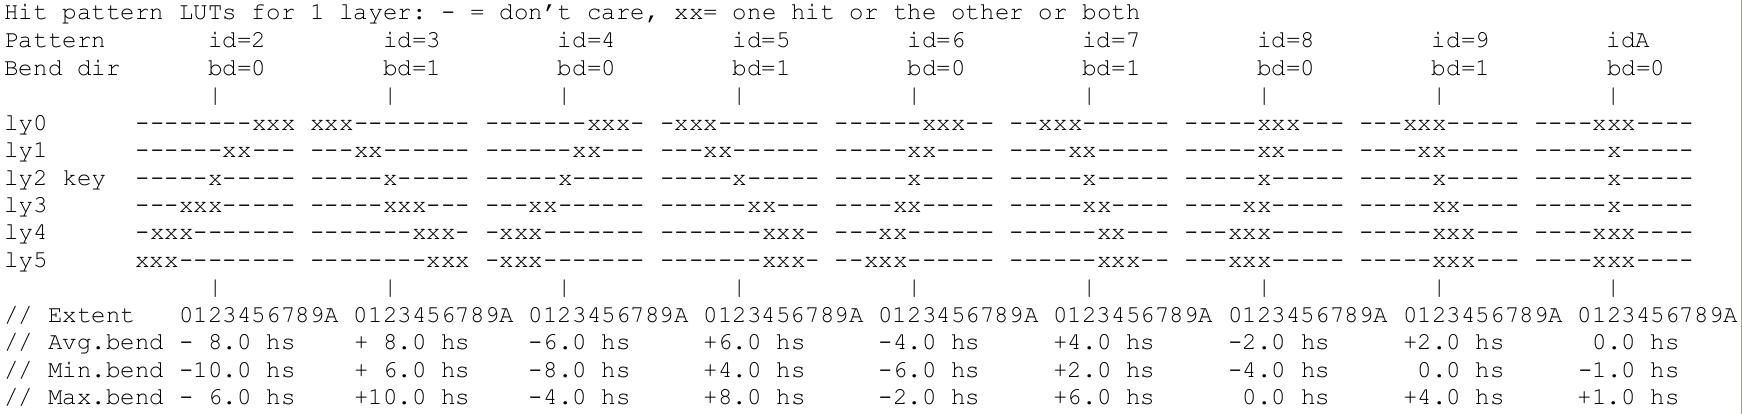
\includegraphics[width=0.98\linewidth]{figures/CLCT_patterns.png}
                \caption{CLCT patterns}
                \label{fig:clct_patterns}
        \end{center}
\end{figure}

Pattern ID=1 is a layer-OR trigger, Pattern ID=0 is no-pattern-found. Result for each of 160 keys is a list of 9 pattern-ID numbers (pid) [2 to A] and corresponding
number of layers [0 to 6] with matching hits (nhits). Find the best 1-of-9 pattern ID numbers for each key by comparing nhits. Ignore bend direction: left and right bends have equal priority (bit 0 of pid implies bend direction).
If two pattern IDs have the same nhits, take the higher pattern ID. A key with no matching hits, would always return pid=A and nhits=0.
Pre-trigger if any 1-of-160 keys have nhits $\geq$ hit\_thresh\_pretrig and pid $\geq$ pid\_thresh\_pretrig.

Construct 7-bit pattern quality pat[7:0] for sorting where pat[7:5]=nhits[2:0], pat[4:0]=pid[3:0]. Ignore the bend direction bit (pid[0]), left and right bends have equal priority. 
Store pat[7:0] for 160 keys for use later to find 2nd CLCT.
Find the best key out 1-of-160 keys by sorting on the 6-bit number pat[7:1]. Store 1st CLCT info: key, pattern ID, and number of hits.
For empty events, key=0, pid=A and nhits=0. If clct\_blanking=1, then key=pid=hits=0.

Mark keys near 1st CLCT as busy from 1st key-nspan to 1st key+pspan.
If clct\_sep\_src=1, pspan and nspan are set equal to clct\_sep\_vme, typically 10 half-strips.
If clct\_sep\_src=0, pspan and nspan are read from RAM and depend on the pattern ID number, this allows two less bending tracks to be closer than more bending tracks.

Find the best key out of 1-of-160 keys by sorting on the 6-bit number pat[7:1]: skip busy keys, if two keys have the same pat[7:1] take the lower key.
Store the same information for the 2nd CLCT as for the 1st one.

Wait for CSC drifting (drift delay of 2BXs) and perform matching to ALCTs.

\newpage
\subsection{Software Emulation of CLCT Processing}

CLCT processing includes the following four steps:

\begin{itemize}
    \item Pulse extension;
    \item Pretrigger;
    \item Trigger;
    \item CLCT construction and CLCT dead time.
\end{itemize}

In contrast to ALCT processing, where all steps are independent and performed one after another for all 16 BXs, during CLCT processing last three steps repeated in one global loop over BXs.

\subsubsection{Pulse Extension}

Sofware emulation provides information about all half-strip signals in DAQ readout window (16 BXs). A search for these signals is performed in a loop over all half-strips, all layers, and all 16 BXs; found signals are stretched over 6 BXs (see Fig.~\ref{fig:clct_pulse_extension}).

\begin{figure}[tbh]
        \begin{center}
                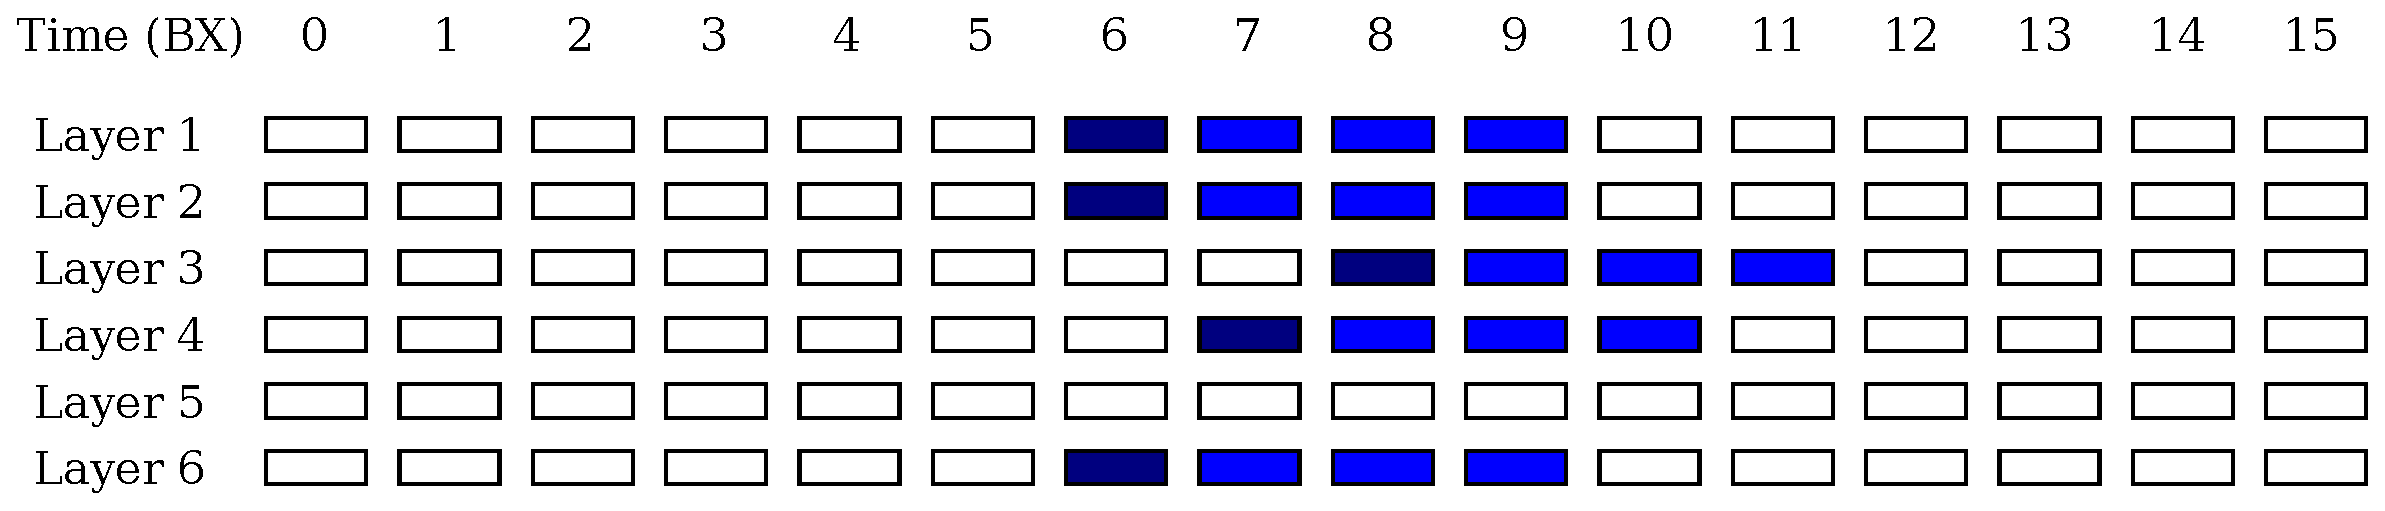
\includegraphics[width=0.9\linewidth]{figures/stretched_hits_clct.pdf}
                \caption{Illustration of ALCT pulse extension for one specific half-strip.}
                \label{fig:clct_pulse_extension}
        \end{center}
\end{figure}

\subsubsection{Pretrigger}

After all available half-strip signals are stretched, start a global loop over all BXs from BX = 0 and search for CLCT pretriggers in all half-strips. For any given BX and half-strip, count the number of layers with hits within the patterns shown on Fig.~\ref{fig:clct_pretrigger}, and if this number is greater than or equal to three, then we say that a pretrigger occured in this BX and this half-strip. This pretrigger is only accepted if its pattern id $\geq$ 2. If there were no CLCTs found in some BX = B, proceed to BX = B+1 and continue searching for pretriggers. If there are some CLCTs found in the current BX, proceed to next step.

\begin{figure}[tbh]
        \begin{center}
                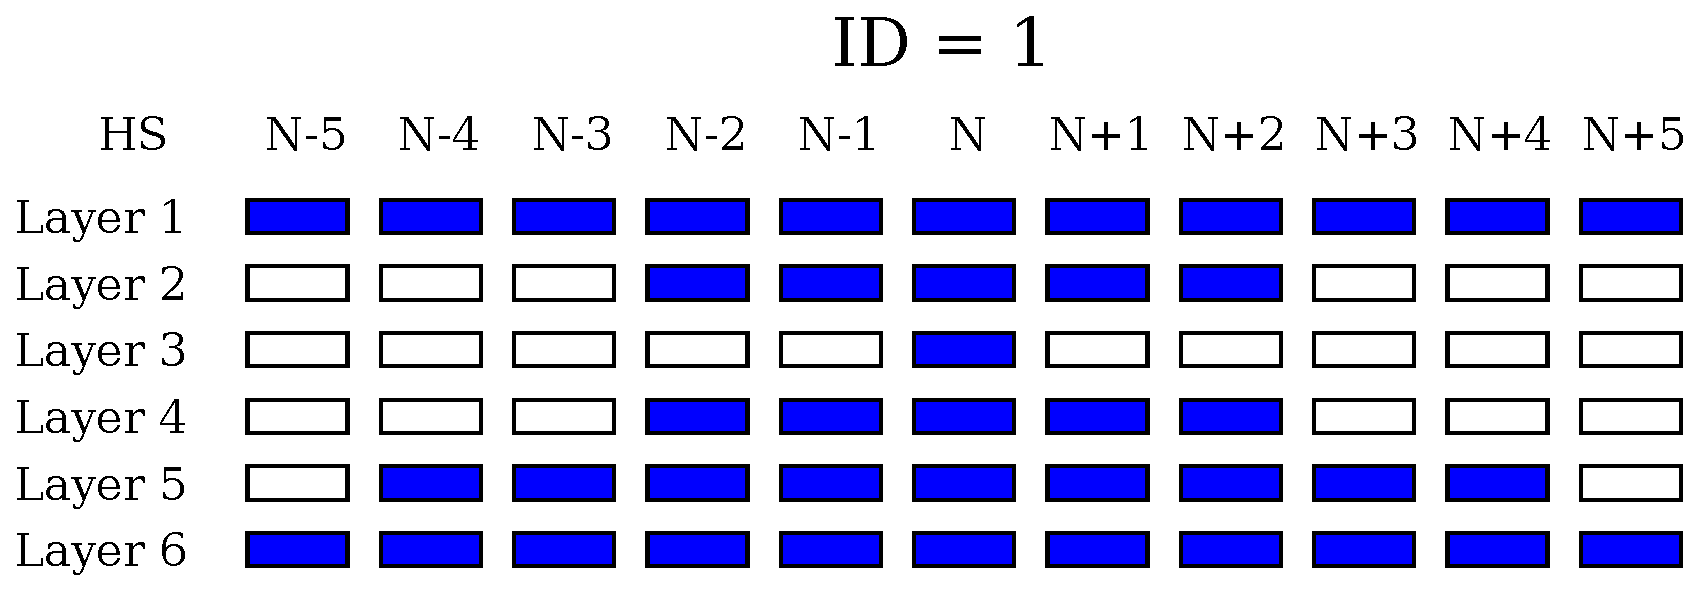
\includegraphics[width=0.48\linewidth]{figures/clct_pattern_01.pdf}
                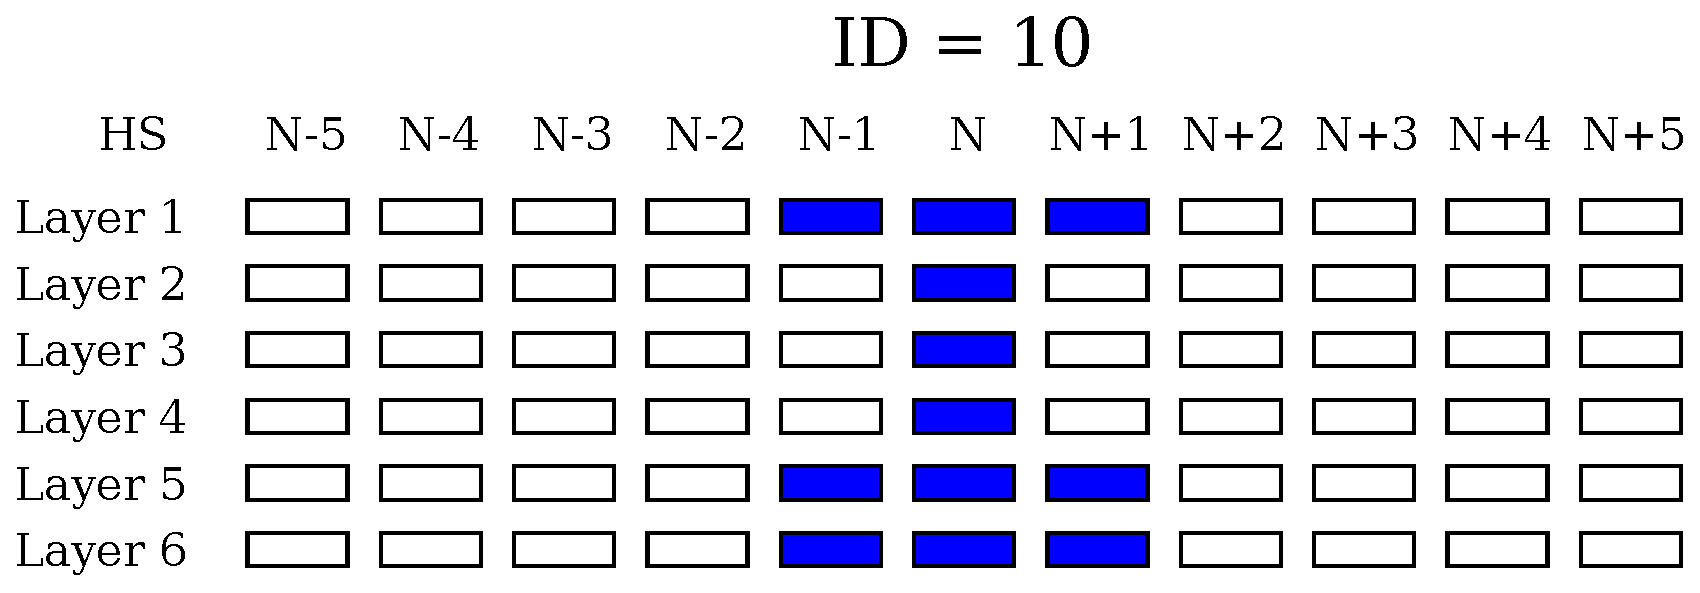
\includegraphics[width=0.48\linewidth]{figures/clct_pattern_10.pdf}\\
                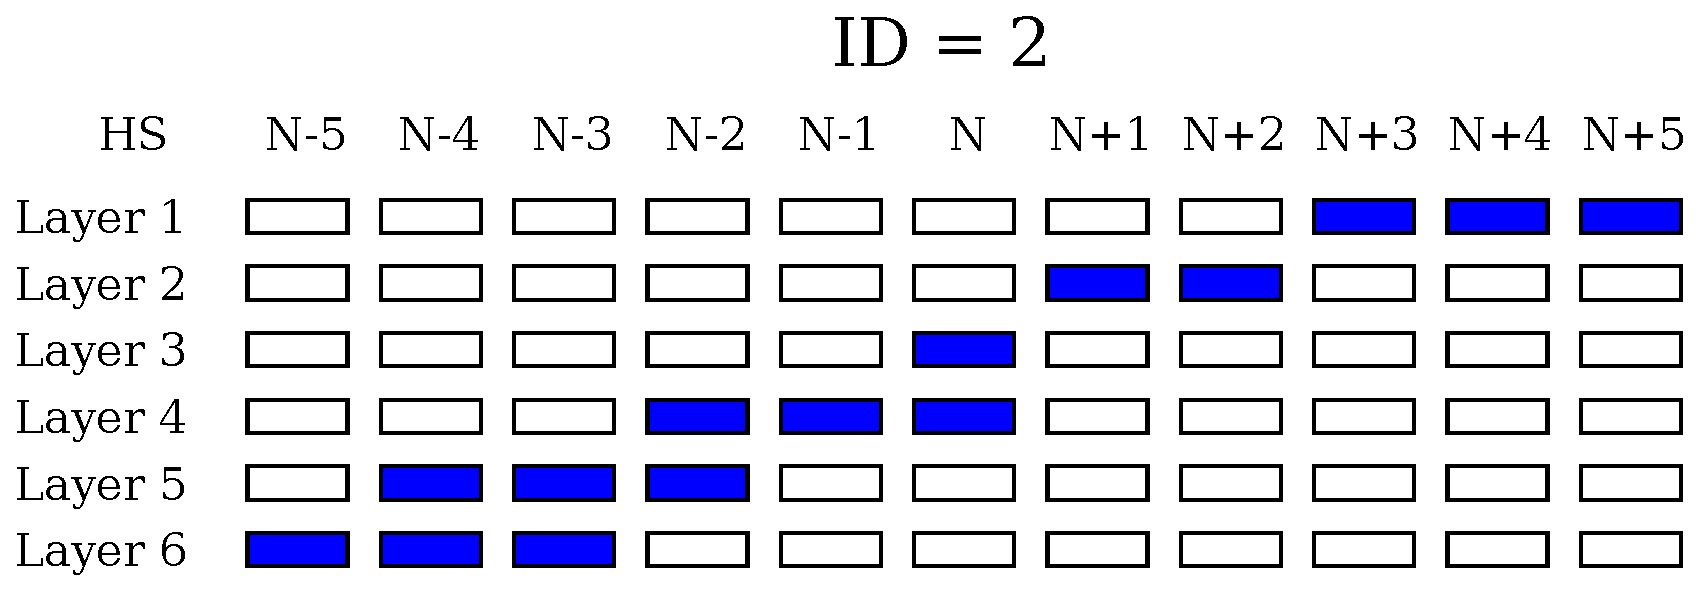
\includegraphics[width=0.48\linewidth]{figures/clct_pattern_02.pdf}
                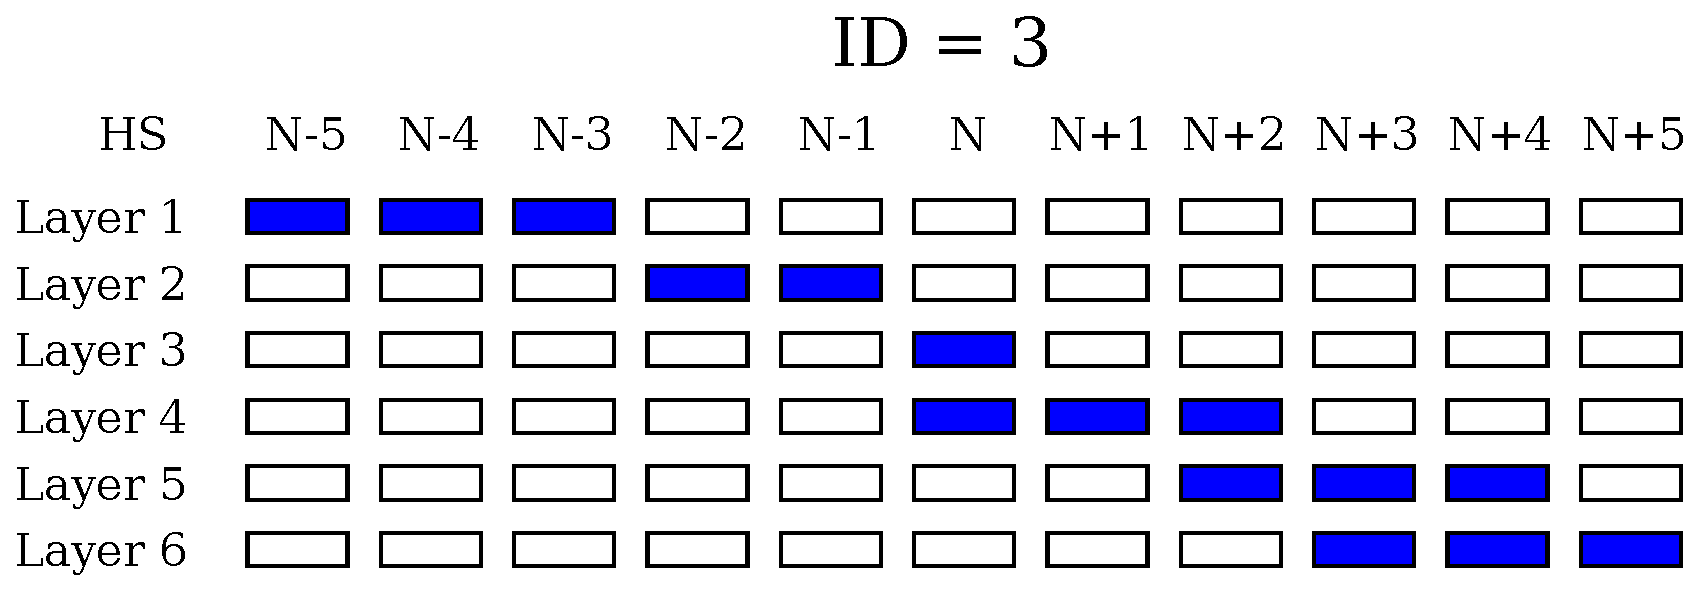
\includegraphics[width=0.48\linewidth]{figures/clct_pattern_03.pdf}\\
                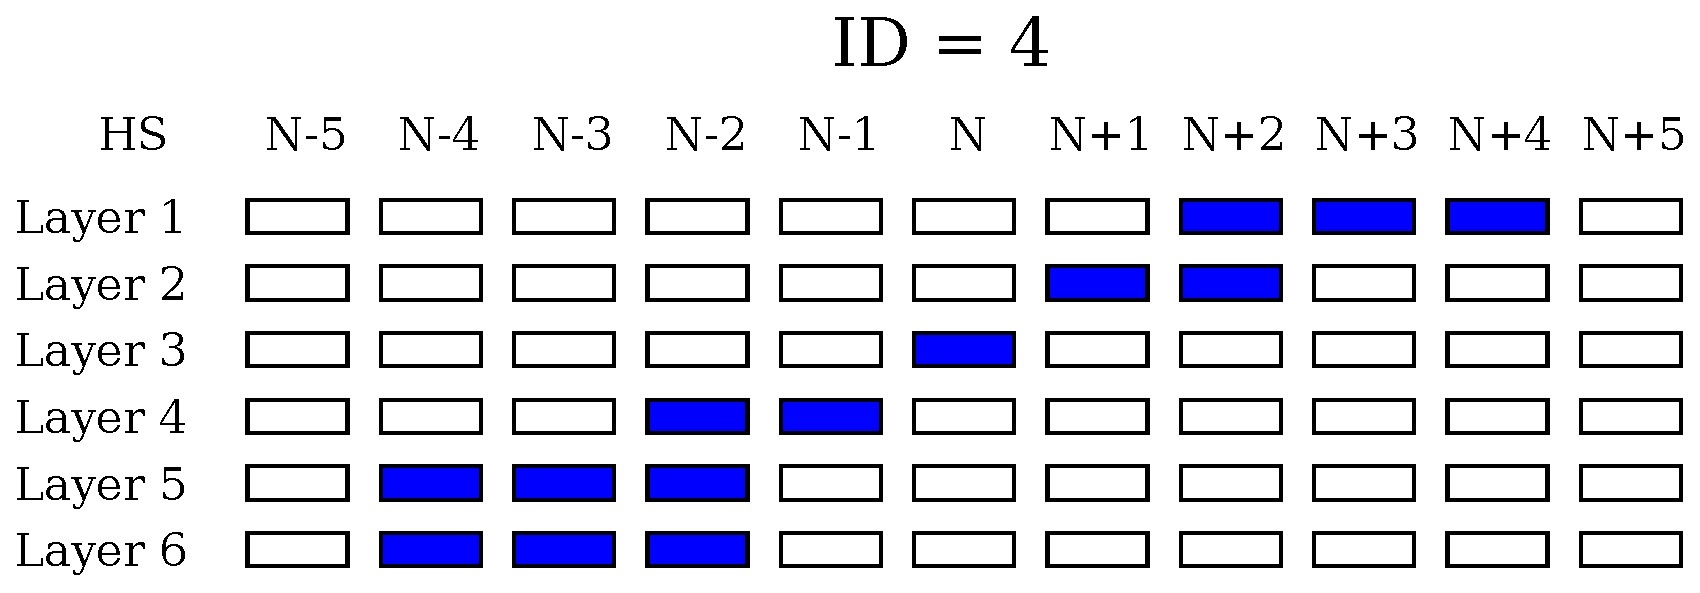
\includegraphics[width=0.48\linewidth]{figures/clct_pattern_04.pdf}
                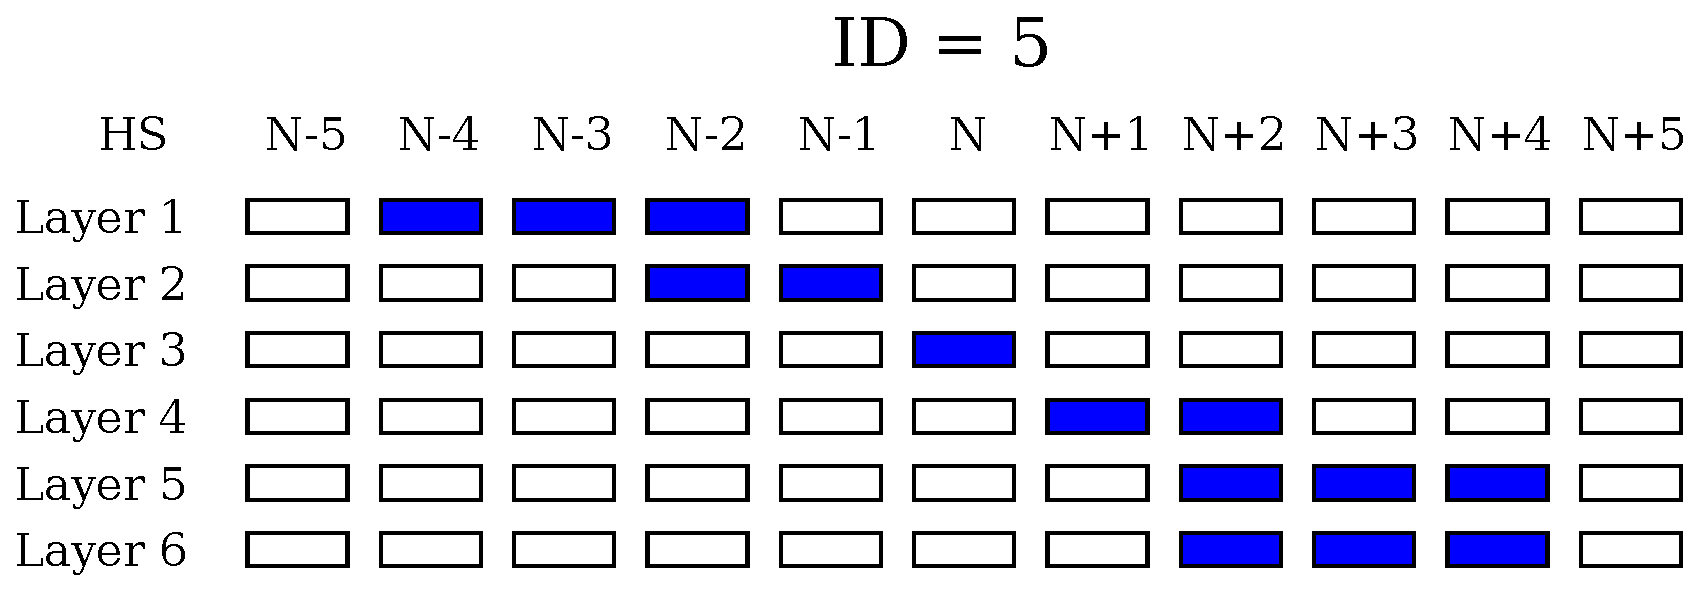
\includegraphics[width=0.48\linewidth]{figures/clct_pattern_05.pdf}\\
                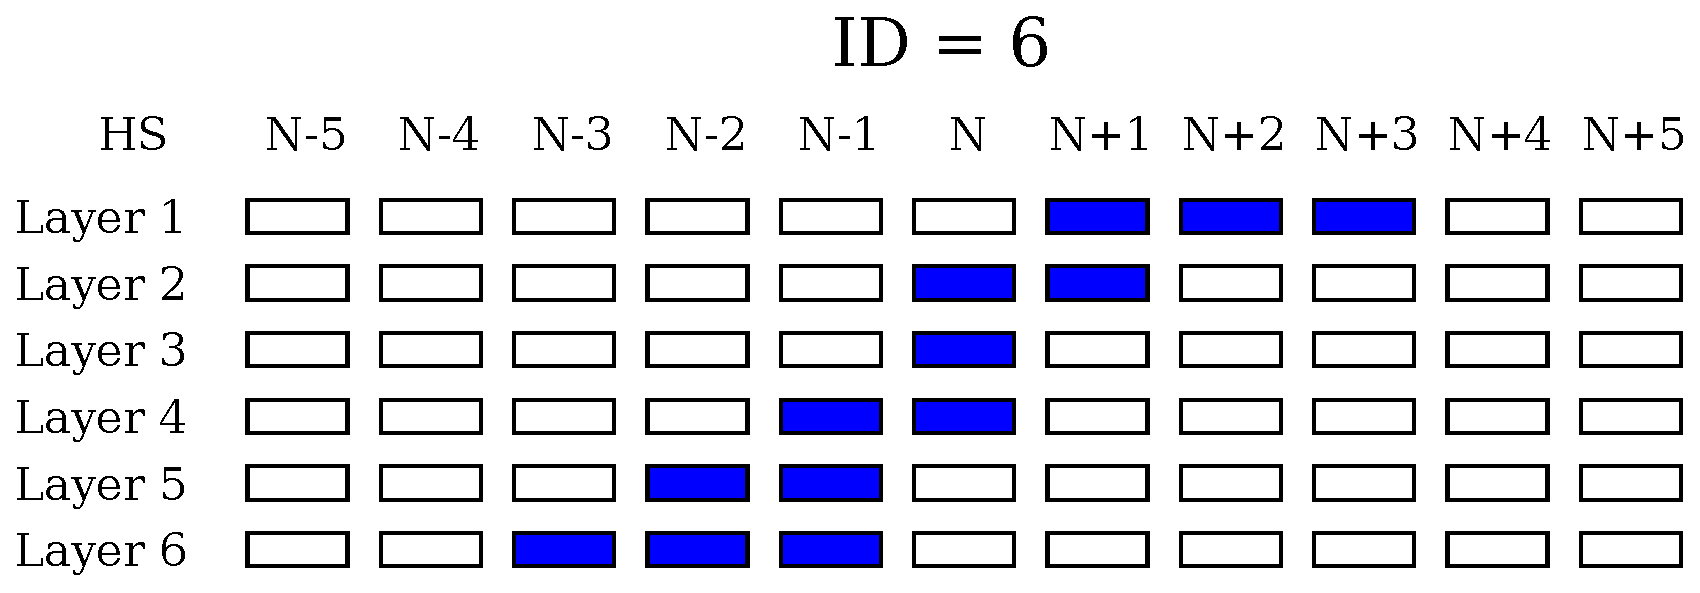
\includegraphics[width=0.48\linewidth]{figures/clct_pattern_06.pdf}
                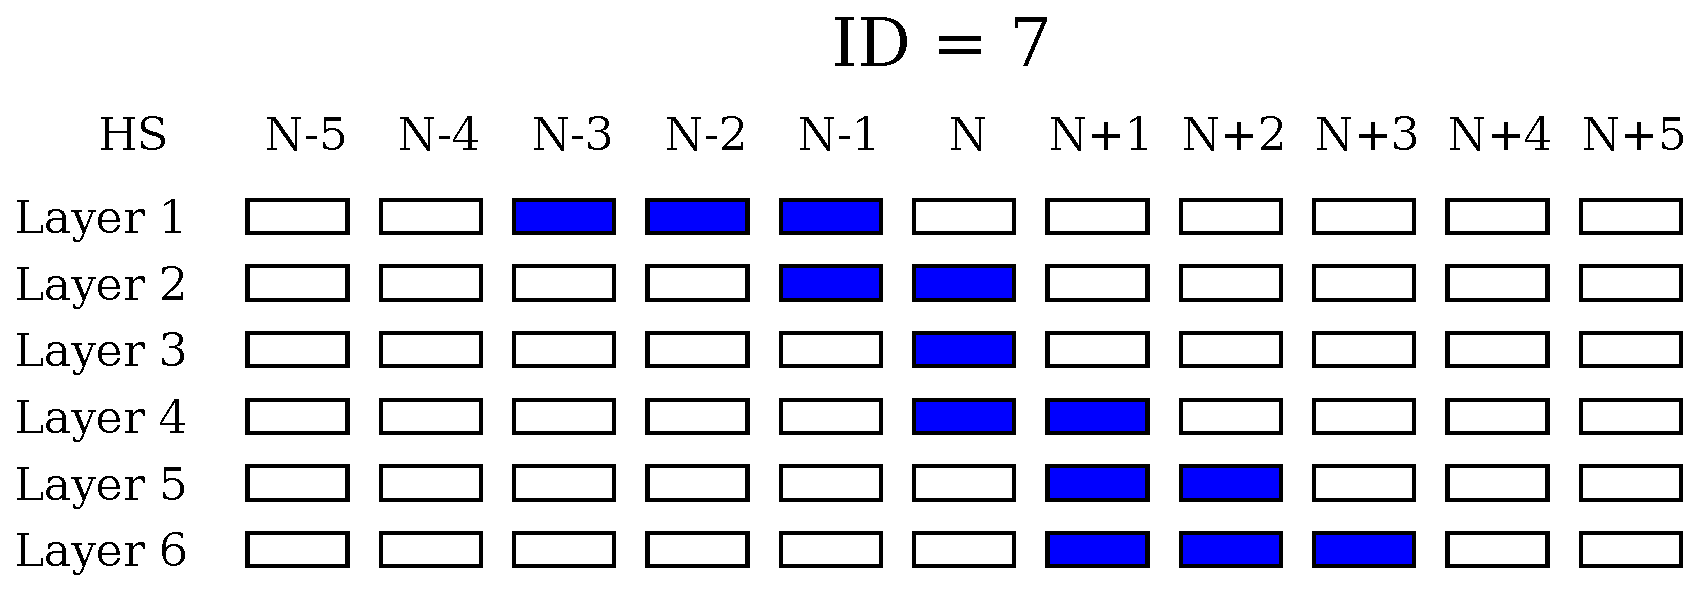
\includegraphics[width=0.48\linewidth]{figures/clct_pattern_07.pdf}\\
                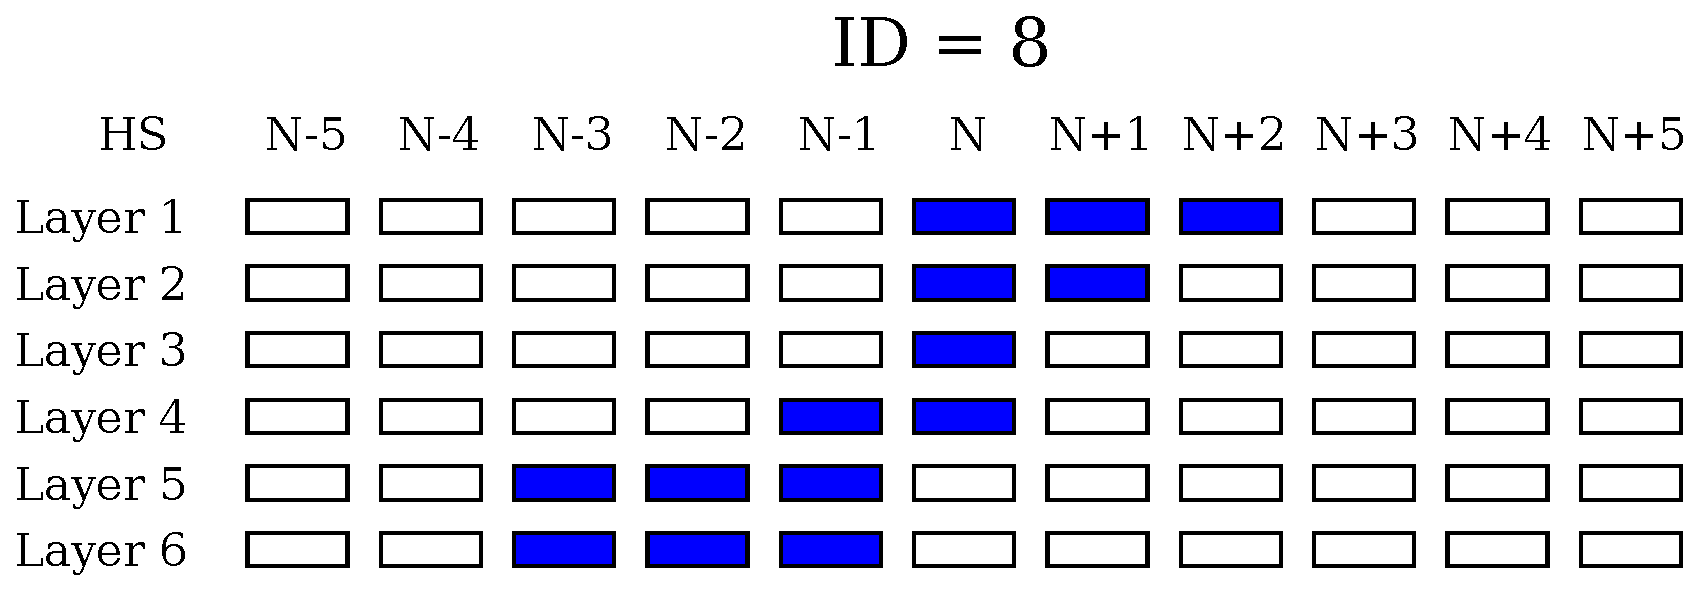
\includegraphics[width=0.48\linewidth]{figures/clct_pattern_08.pdf}
                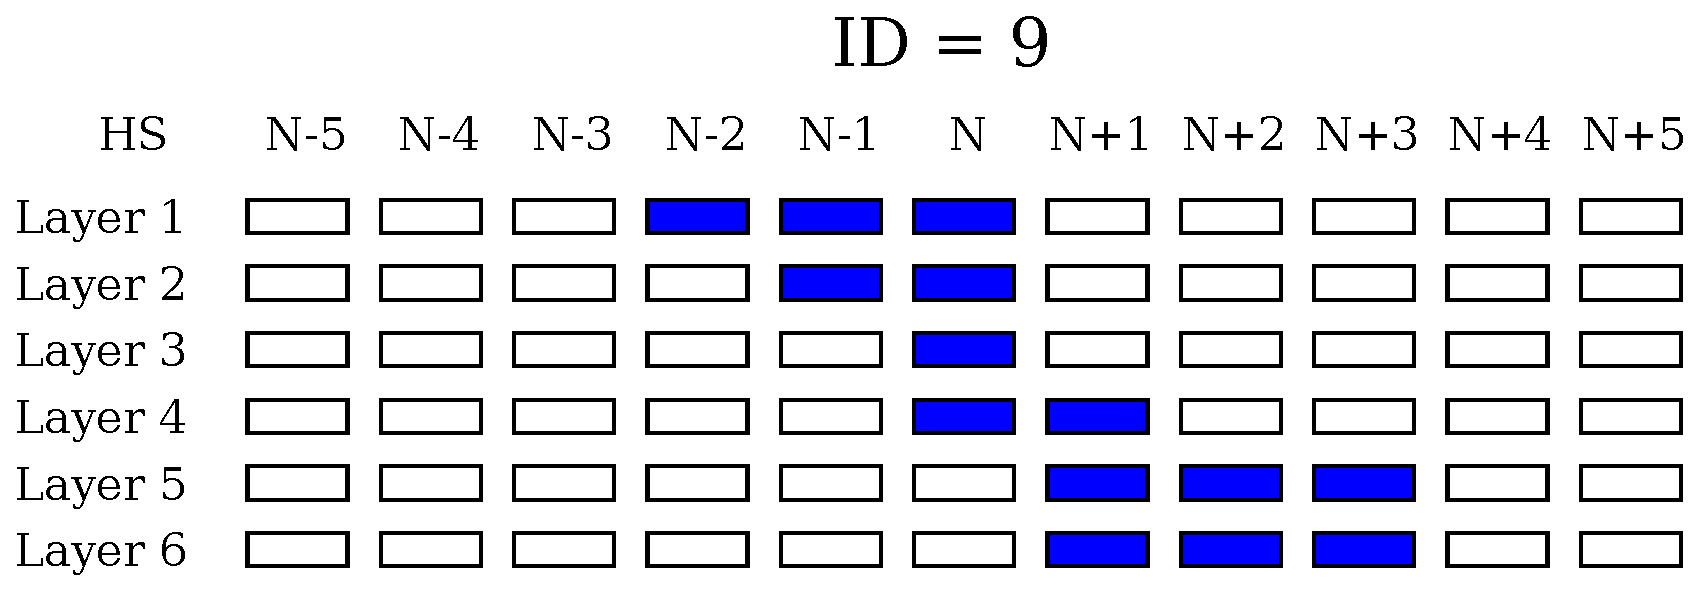
\includegraphics[width=0.48\linewidth]{figures/clct_pattern_09.pdf}
                \caption{CLCT patterns for pretriggering and triggering.}
                \label{fig:clct_pretrigger}
        \end{center}
\end{figure}

\subsubsection{Trigger}

As soon as a BX = B with CLCT pretrigger(s) is found, search for triggers in BX = B+2. For each half-strip, count the number of layers with hits within the same patterns used for pretriggering, and if this number is greater than or equal to four, we say that a trigger occured in this half-strip and BX, and remember:
\begin{itemize}
    \item pattern id with the highest number of hit layers (if there are two pattern ids with the same number of hit layers, choose smaller pattern id);
    \item number of hit layers in this pattern id.
\end{itemize}

Proceed to next step.

\subsubsection{CLCT Construction and CLCT Dead Time}

In a BX with CLCT triggers, find up to two best triggers to be used in CLCT construction.

Find the best trigger:
\begin{itemize}
    \item Find trigger with the highest number of hit layers;
    \item If there are two triggers with the same number of hit layers: choose the one with higher pattern id;
    \item If there are two triggers with the same number of hit layers and the same pattern id: choose the one with smaller half-strip.
\end{itemize}

Mark zone of 20 half-strips around the best trigger as used and find the second best trigger among not used half-strips.

Construct up to two best CLCTs from found best triggers: encode quality, pattern, bending direction, half-strip, cfeb, BX (defined by pretrigger BX).

After CLCT construction, keep CLCT "dead": continue the loop over all BXs until there is a BX with no triggers. When such a BX is found go back to pretriggering step.

\newpage
\subsection{CLCT and ALCT Correlation}

The Trigger Motherboard (TMB) portion of the CLCT/TMB card receives up to two
anode stubs from the ALCT board and two cathode stubs from the CLCT portion of the CLCT/
TMB card. The functions of the TMB circuitry are:

\begin{itemize}
	\item Bunch crossing alignment of the anode and cathode tags.
	\item Correlation of the Anode and Cathode LCT words and construction of two combined LCTs.
	\item Transmission of LCT data to the Muon Port Card (MPC) for triggering, and transmission of DAQ data to the DAQ Motherboard (DAQMB).
\end{itemize}

Incoming anode and cathode LCTs are not aligned in time. Anode LCTs are created
faster than cathode LCTs because of the slow development of the cathode preamp signal, and
because processing inside the ALCT card is faster than processing inside the CLCT logic. The
TMB contains input pipeline logic in order to delay anode LCTs for a programmable number of
bunch crossings up to 10.

The anode and cathode LCTs are matched according to the more precise ALCT bunch
crossing number (BXN). The Cathode LCT BXN can differ by at most $\pm$1 bunch crossing. For each
of the selected muons the TMB outputs a 2-bit bunch crossing match word as shown in
table below. These may be used by later boards in the trigger chain if additional quality information
is needed. They also allow the analysis of the bunch crossing matching in the TMB, since a large
number of bad matches could be an indication of a timing alignment problem.

The ideal case for a high-momentum muon is one anode and one cathode LCT pattern.
However, other cases may occur, which are distinguished by a 2-bit “STA” (Status type A) code:

\begin{itemize}
	\item The TMB may receive one or two anode LCTs and zero cathode LCT patterns. This
happens, for example, for very low-momentum muons. Although the non-zero data is
forwarded to the MPC, this case is flagged by STA=1, as is the similar case of one or two
cathode LCT and zero anode LCT patterns.
	\item If the TMB receives two anode LCTs and one cathode LCT, the TMB outputs two LCTs,
by copying the Cathode LCT bits into both muons. These, and the similar case of two
cathode LCTs and one anode LCT, are flagged by STA=2.
	\item If there are two anode LCTs and two cathode LCTs in one chamber, they are matched
according to their pattern numbers: the largest ALCT and CLCT pattern numbers are
paired, and the second largest ALCT and CLCT pattern numbers are paired. These, and
the ideal case of a single match, are flagged by STA=3.
\end{itemize}

TMBs maintain a local Bunch Crossing Number (BXN) using signals from the Clock
and Control Board. The internal BXN is compared to the BXN received from the ALCT module,
and the Sync Error bit is set if a mismatch is detected.

The TMB sends up to two anode LCT and two cathode LCT patterns for one CSC
chamber to the MPC every 25 ns.

\newpage
\subsection{Software Emulation of CLCT and ALCT Correlation}

Every BX OTMB receives up to 2 CLCTs and up to two ALCTs from CLCT and ALCT processors, Fig.~\ref{fig:clcts_alcts} shows an example which will be used throughout the subsection.

\begin{figure}[tbh]
        \begin{center}
                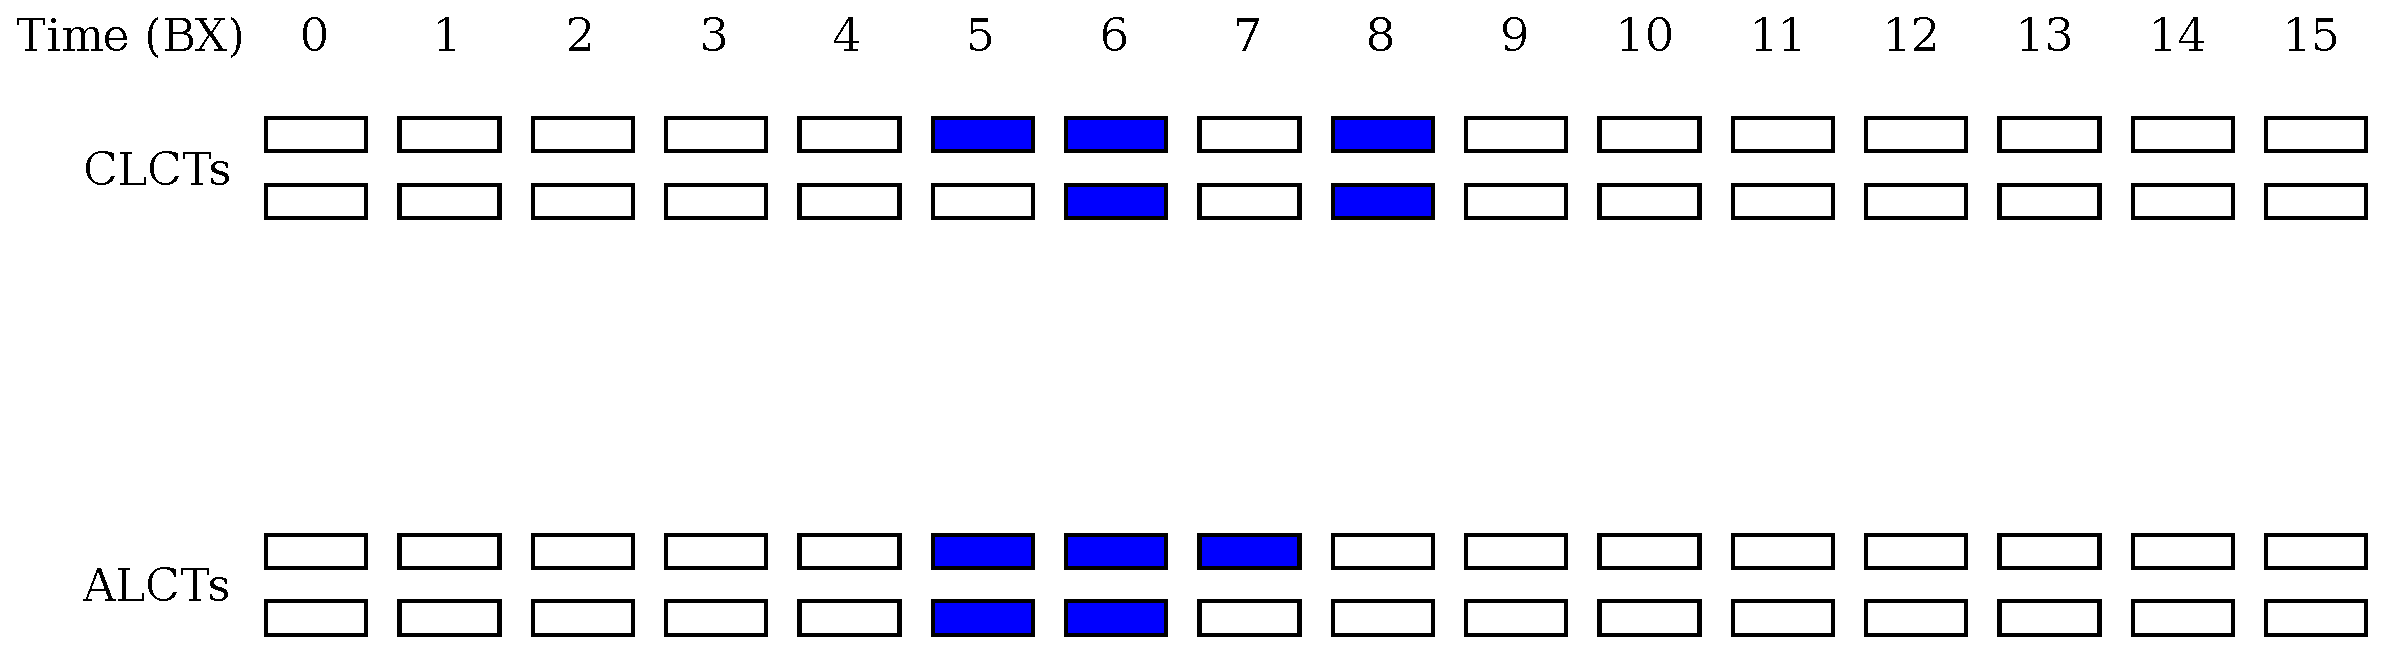
\includegraphics[width=0.7\linewidth]{figures/clcts_alcts.pdf}
                \caption{Example of CLCTs and ALCTs received by OTMB.}
                \label{fig:clcts_alcts}
        \end{center}
\end{figure}

There are two approaches to CLCT and ALCT correlation: CLCT-centric and ALCT-centric. We will introduce the former below and discuss the latter later among OTMB level improvements.

CLCT-centric CLCT and ALCT correlation (see Fig.~\ref{fig:clct_alcts}):
\begin{itemize}
    \item Loop over CLCT BXs from BX = 0 to BX = 15
    \item For CLCT BX = B with at least one valid CLCT:
    \begin{itemize}
        \item Loop over ALCT BXs from BX = B-3 to BX = B+3
        \item Find the first ALCT BX in the matching window with at least one valid ALCT and not marked as used before
        \begin{itemize}
            \item Correlate CLCTs and ALCTs in matching ALCT and CLCT BXs
            \item Mark ALCT BX as used
            \item Proceed to next CLCT BX
        \end{itemize}
    \end{itemize}
\end{itemize}

\begin{figure}[tbh]
        \begin{center}
                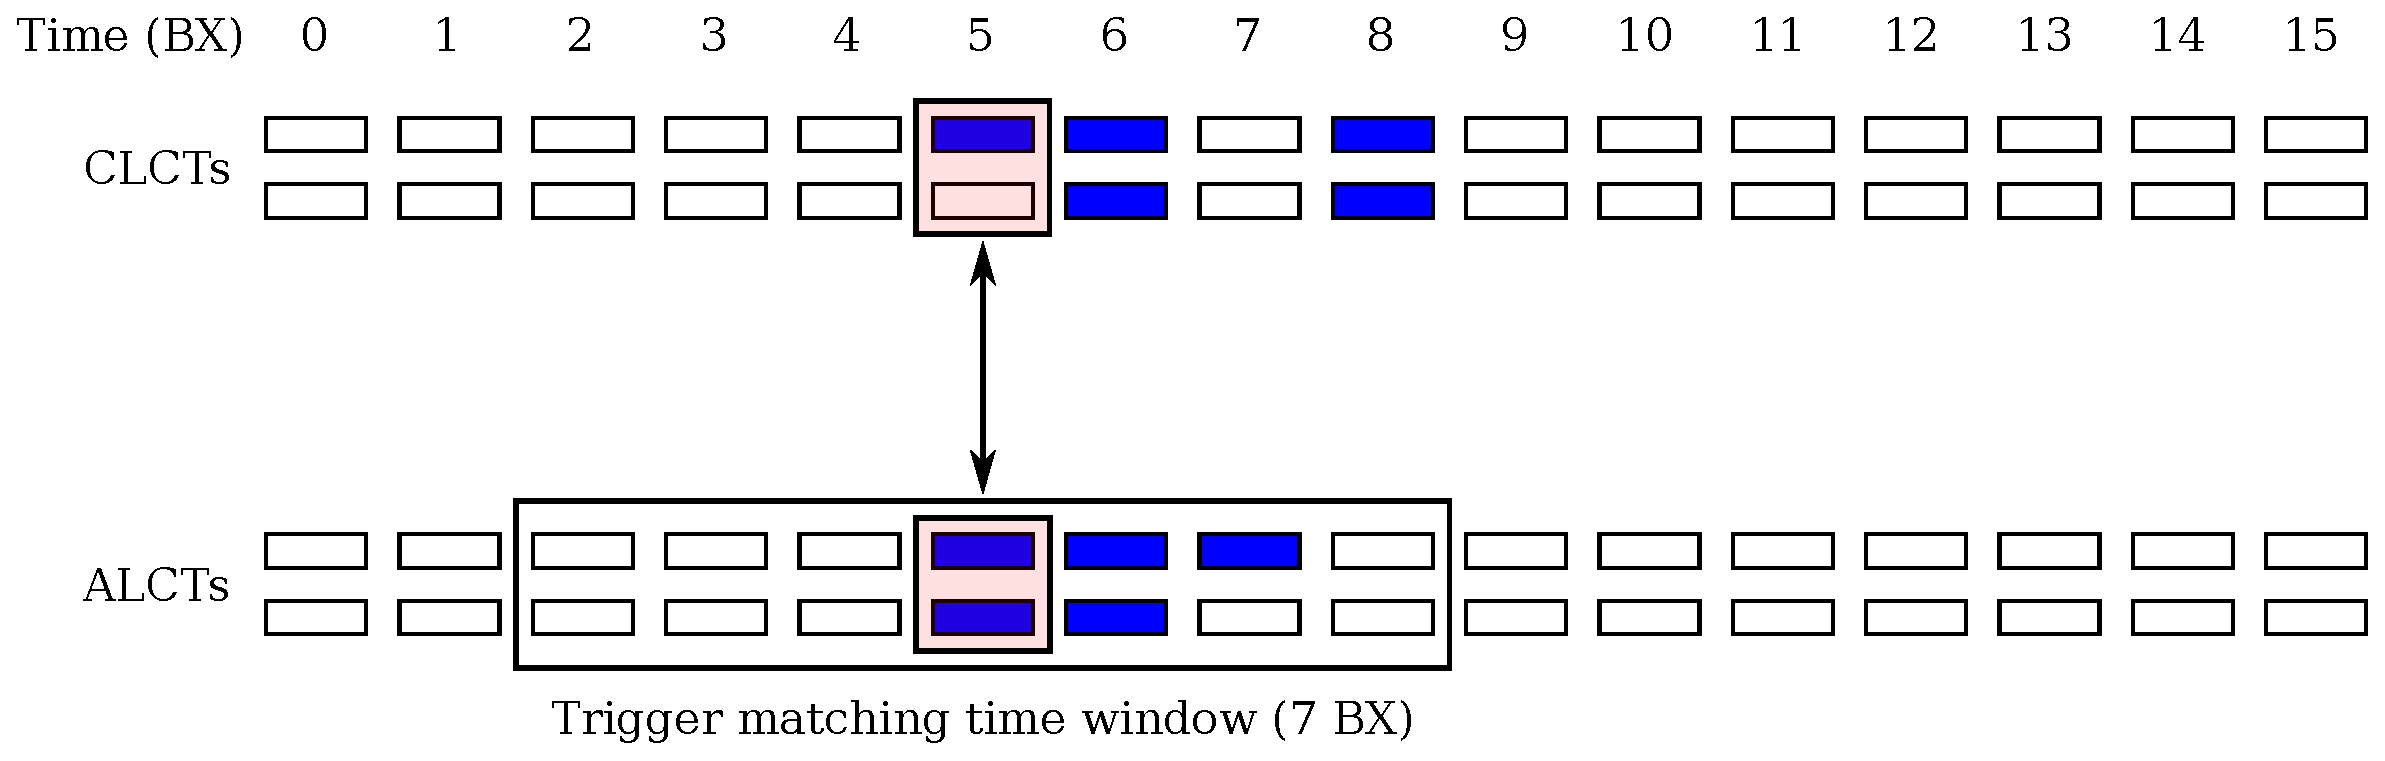
\includegraphics[width=0.7\linewidth]{figures/clct_alcts.pdf}
                \caption{CLCT-centric CLCT and ALCT correlation.}
                \label{fig:clct_alcts}
        \end{center}
\end{figure}

The results of such a correlation are shown on Fig.~\ref{fig:clct_alcts_end}.

\begin{figure}[tbh]
        \begin{center}
                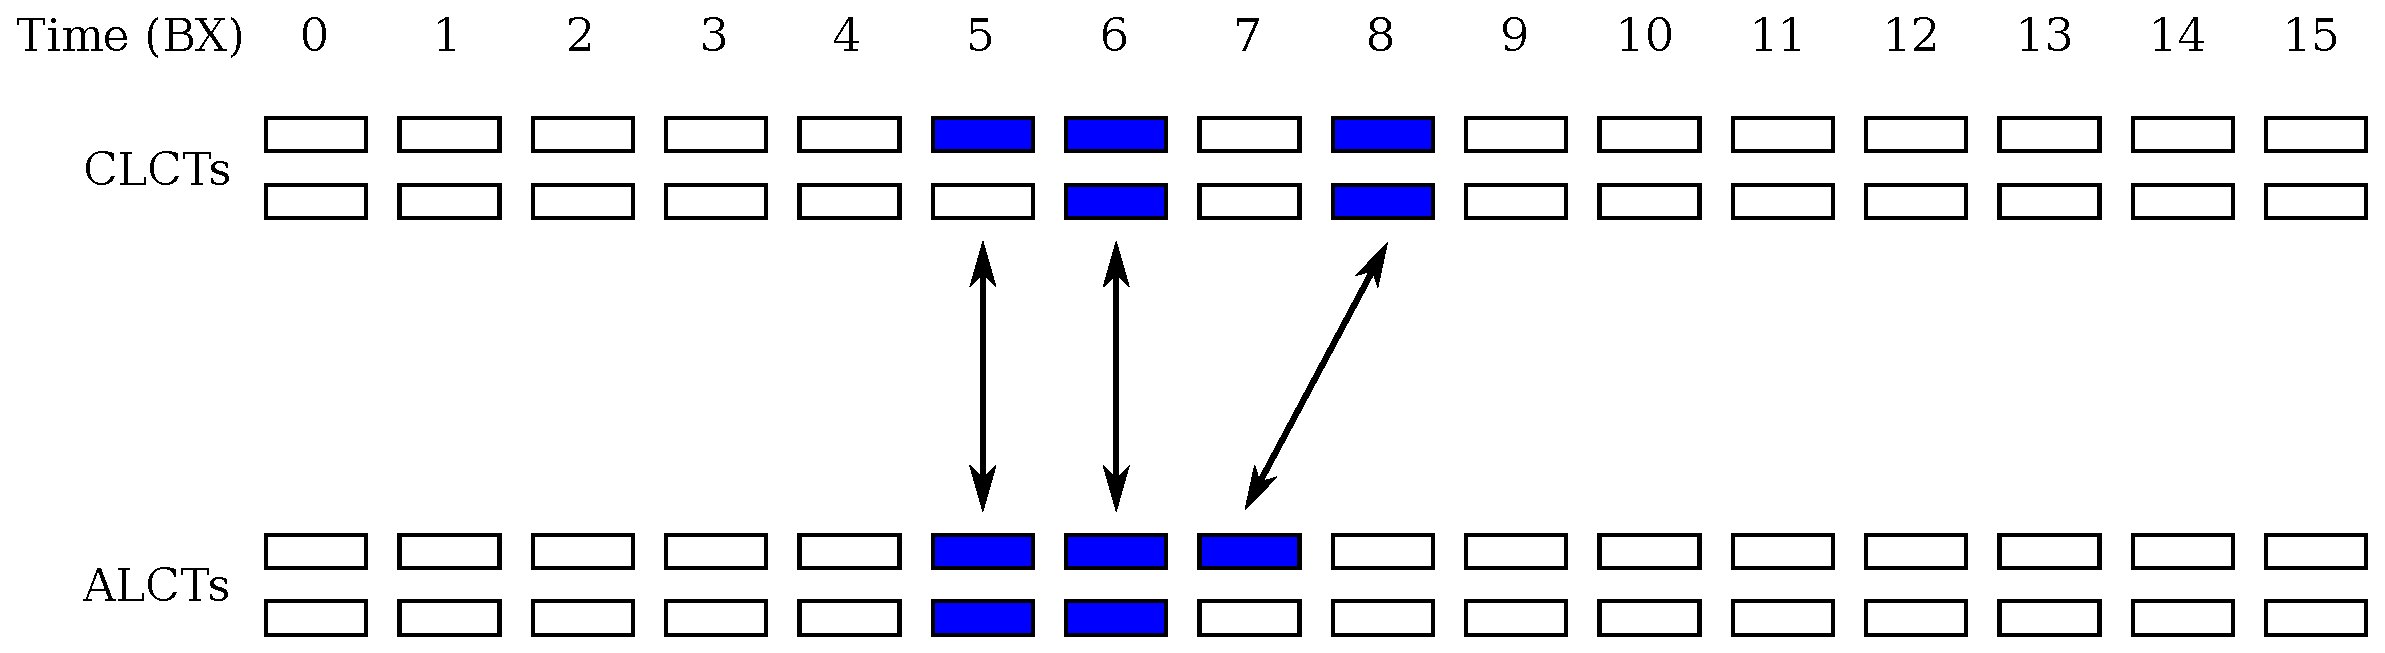
\includegraphics[width=0.7\linewidth]{figures/clct_alcts_end.pdf}
                \caption{Result of CLCT-centric CLCT and ALCT correlation.}
                \label{fig:clct_alcts_end}
        \end{center}
\end{figure}

By default, LCTs are constructed only from valid CLCTs and ALCTs, but we may optionally allow construction of ALCT-less or CLCT-less LCTs.

If there are no ALCT BXs with at least one valid ALCT in the watching window and ALCT-less LCTs are allowed, construct LCTs from valid CLCTs in the current CLCT BX (see example on Fig.~\ref{fig:clct_alcts_alctless} with results on Fig.~\ref{fig:clct_alcts_alctless_end}).

\begin{figure}[tbh]
        \begin{center}
                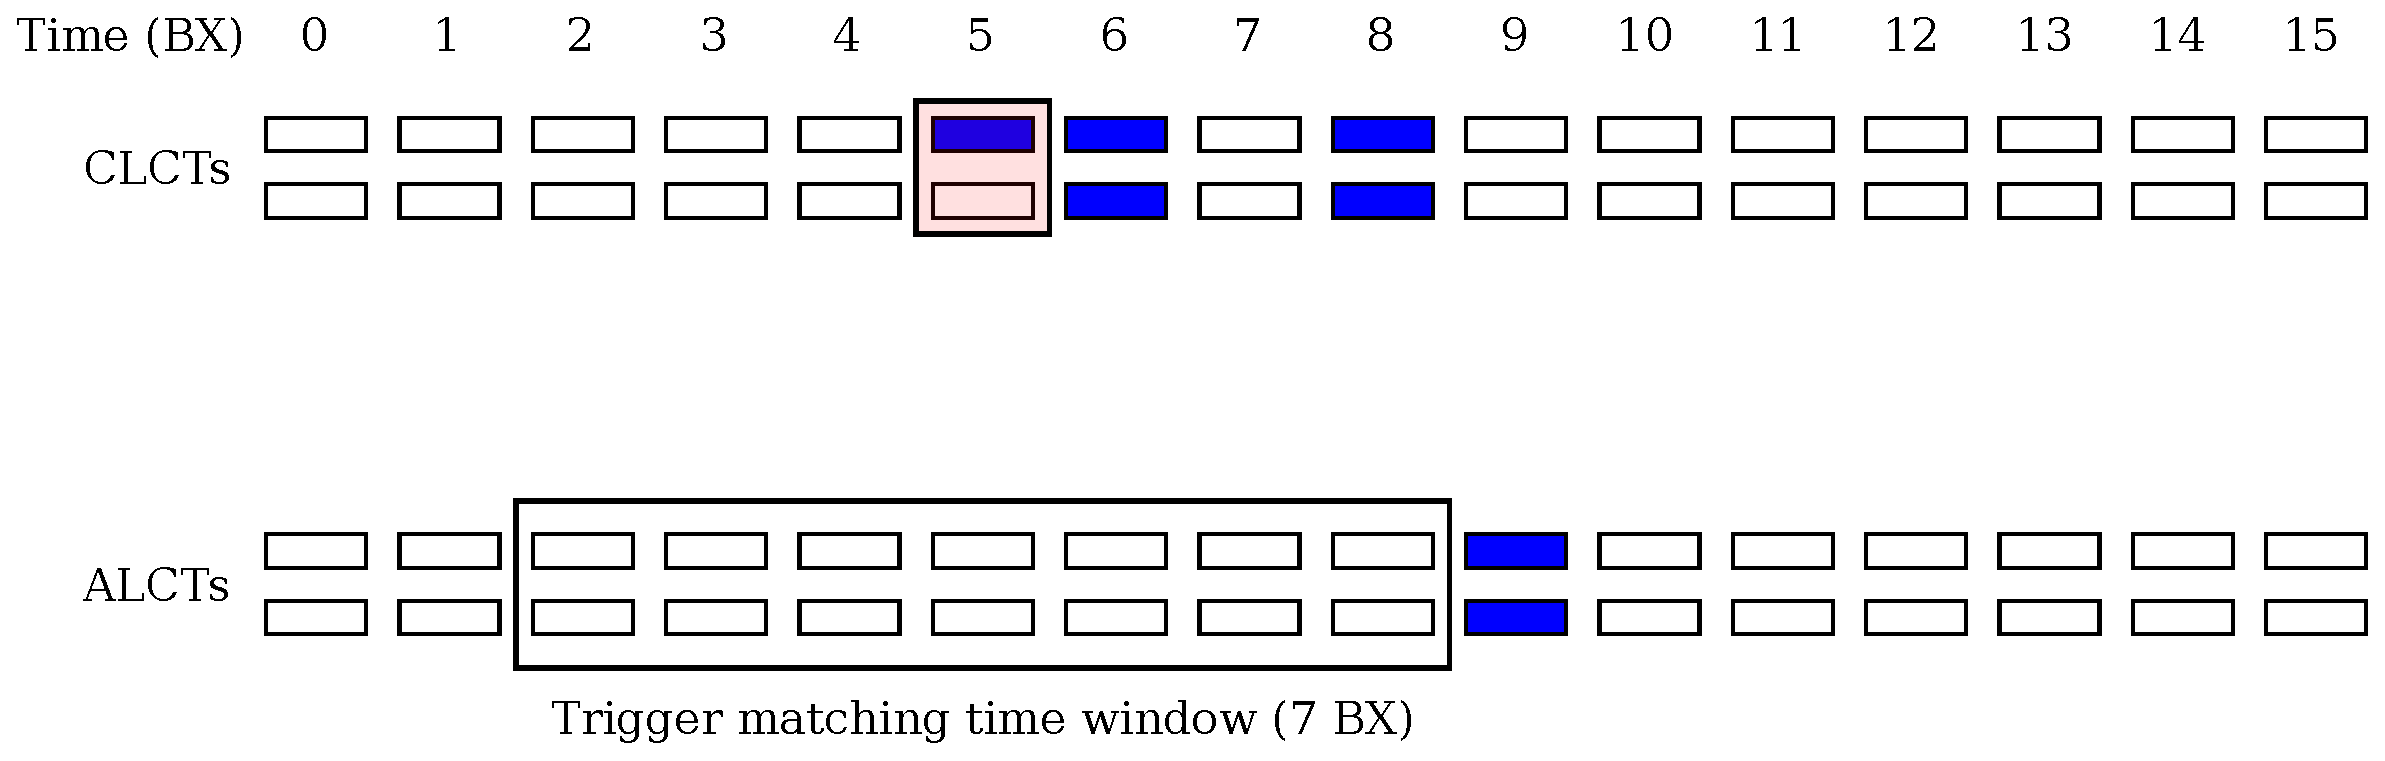
\includegraphics[width=0.7\linewidth]{figures/clct_alcts_alctless.pdf}
                \caption{Example of construction of ALCT-less LCTs.}
                \label{fig:clct_alcts_alctless}
        \end{center}
\end{figure}

\begin{figure}[tbh]
        \begin{center}
                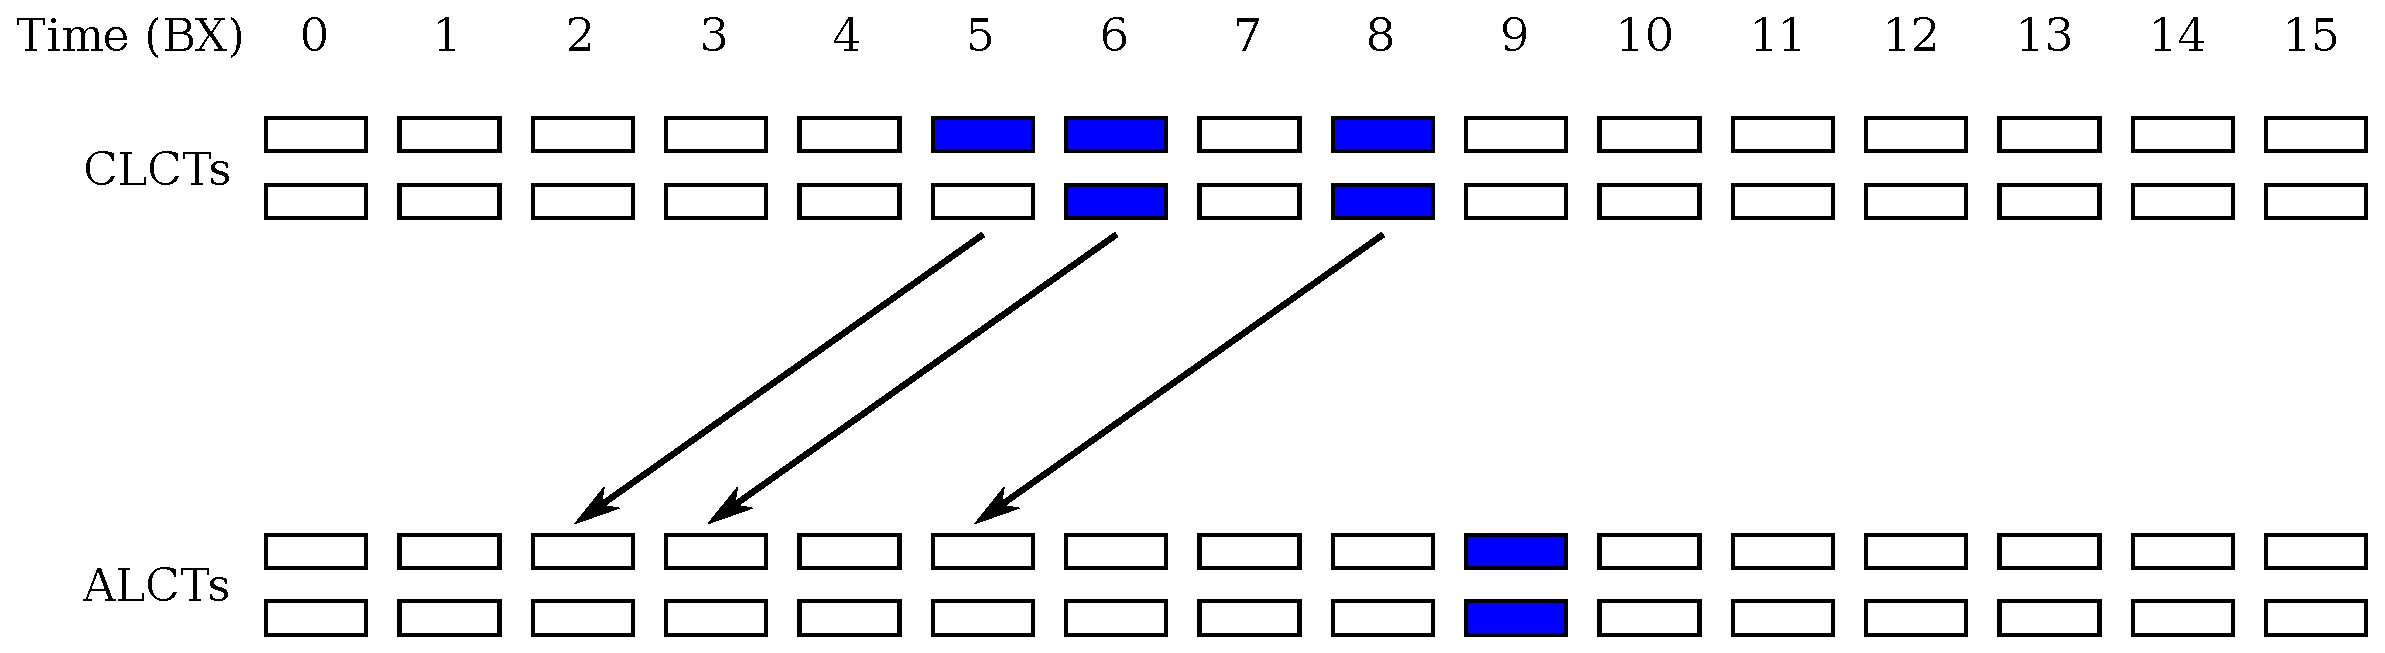
\includegraphics[width=0.7\linewidth]{figures/clct_alcts_alctless_end.pdf}
                \caption{Results of construction of ALCT-less LCTs.}
                \label{fig:clct_alcts_alctless_end}
        \end{center}
\end{figure}

If there are no valid CLCTs in the current CLCT BX and CLCT-less LCTs are allowed (see example on Fig.~\ref{fig:clct_alcts_clctless} with results on Fig.~\ref{fig:clct_alcts_clctless_end}):
\begin{itemize}
    \item Find first ALCT BX in the matching window with at least one valid ALCT and not marked as used before;
    \item Construct LCTs from valid ALCTs in that ALCT BX.
\end{itemize}

\begin{figure}[tbh]
        \begin{center}
                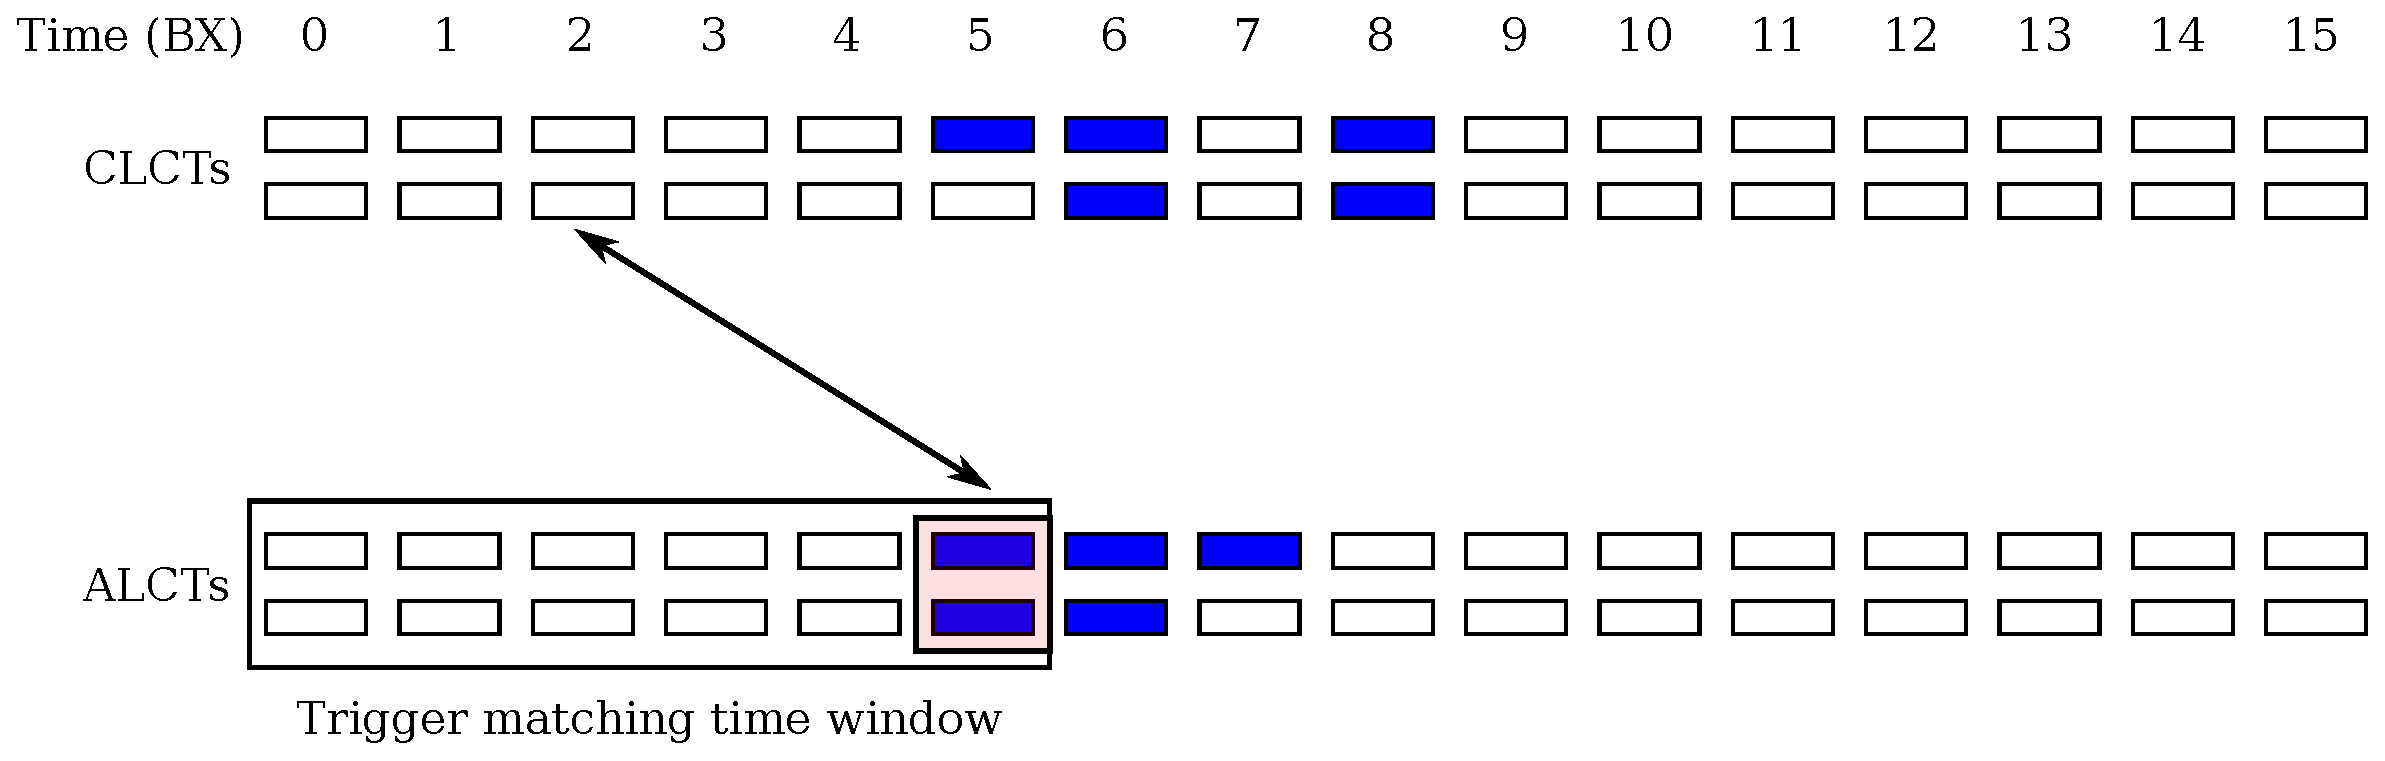
\includegraphics[width=0.7\linewidth]{figures/clct_alcts_clctless.pdf}
                \caption{Example of construction of CLCT-less LCTs.}
                \label{fig:clct_alcts_clctless}
        \end{center}
\end{figure}

\begin{figure}[tbh]
        \begin{center}
                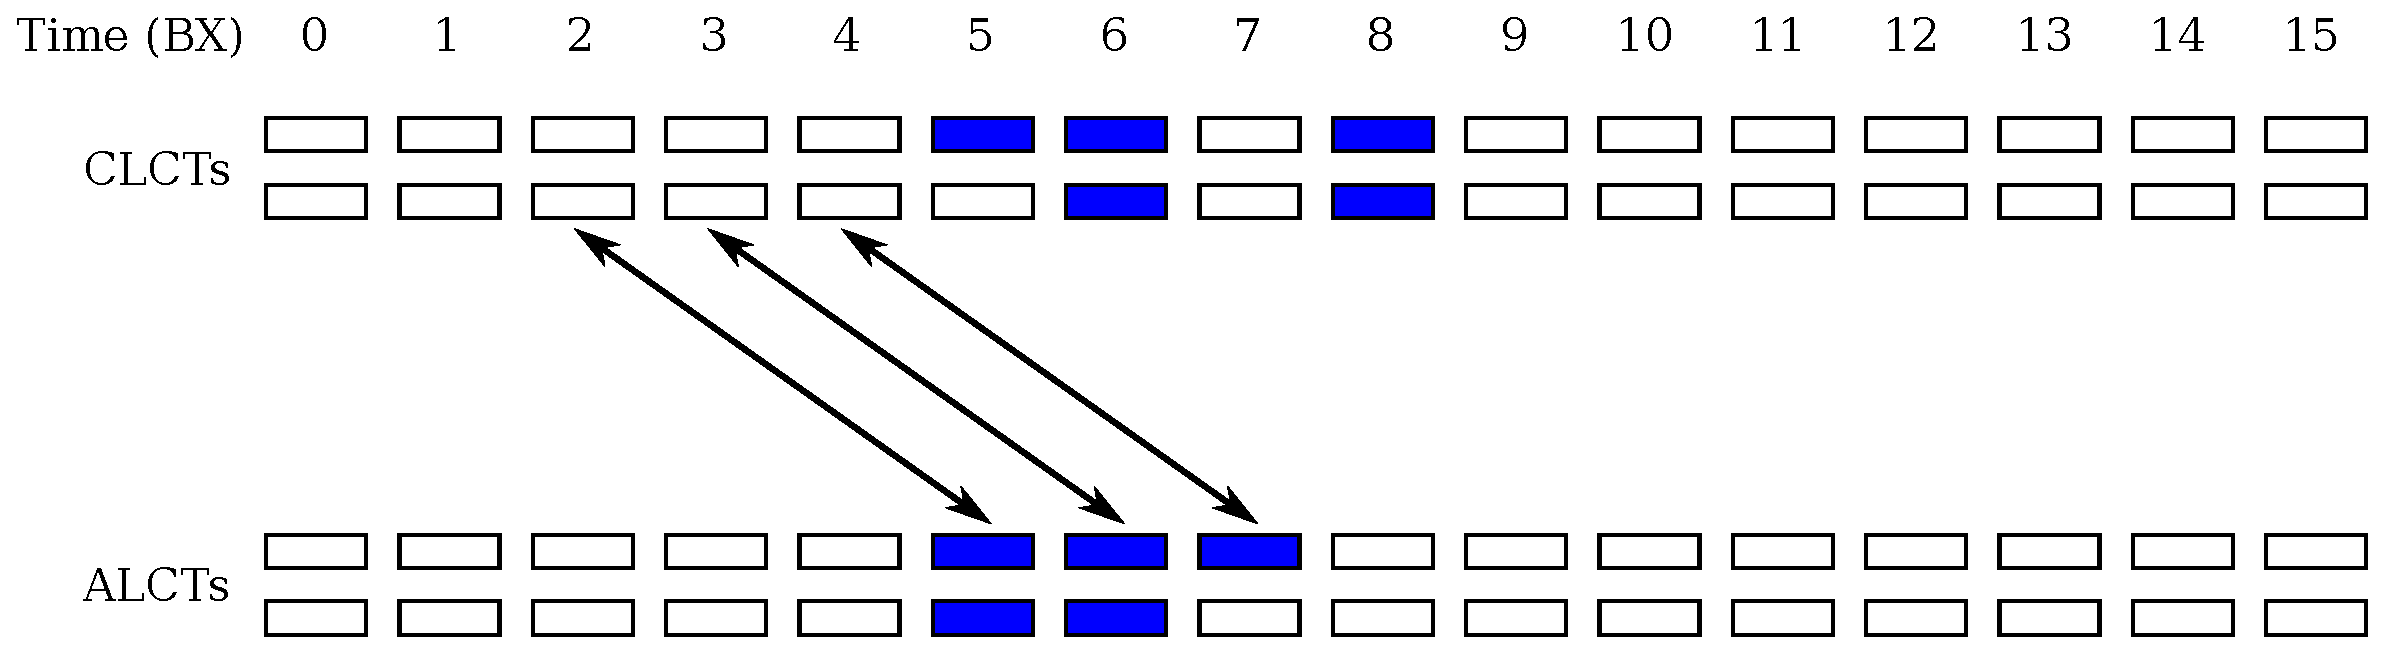
\includegraphics[width=0.7\linewidth]{figures/clct_alcts_clctless_end.pdf}
                \caption{Results of construction of CLCT-less LCTs.}
                \label{fig:clct_alcts_clctless_end}
        \end{center}
\end{figure}

When we use default behavior, where LCTs are constructed only from valid CLCTs and ALCTs, the ideal case is when in matching BXs number of valid CLCTs is equal to number of valid ALCTs (see top two examples on Fig.~\ref{fig:clct_alct_corr}).

\begin{figure}[tbh]
        \begin{center}
                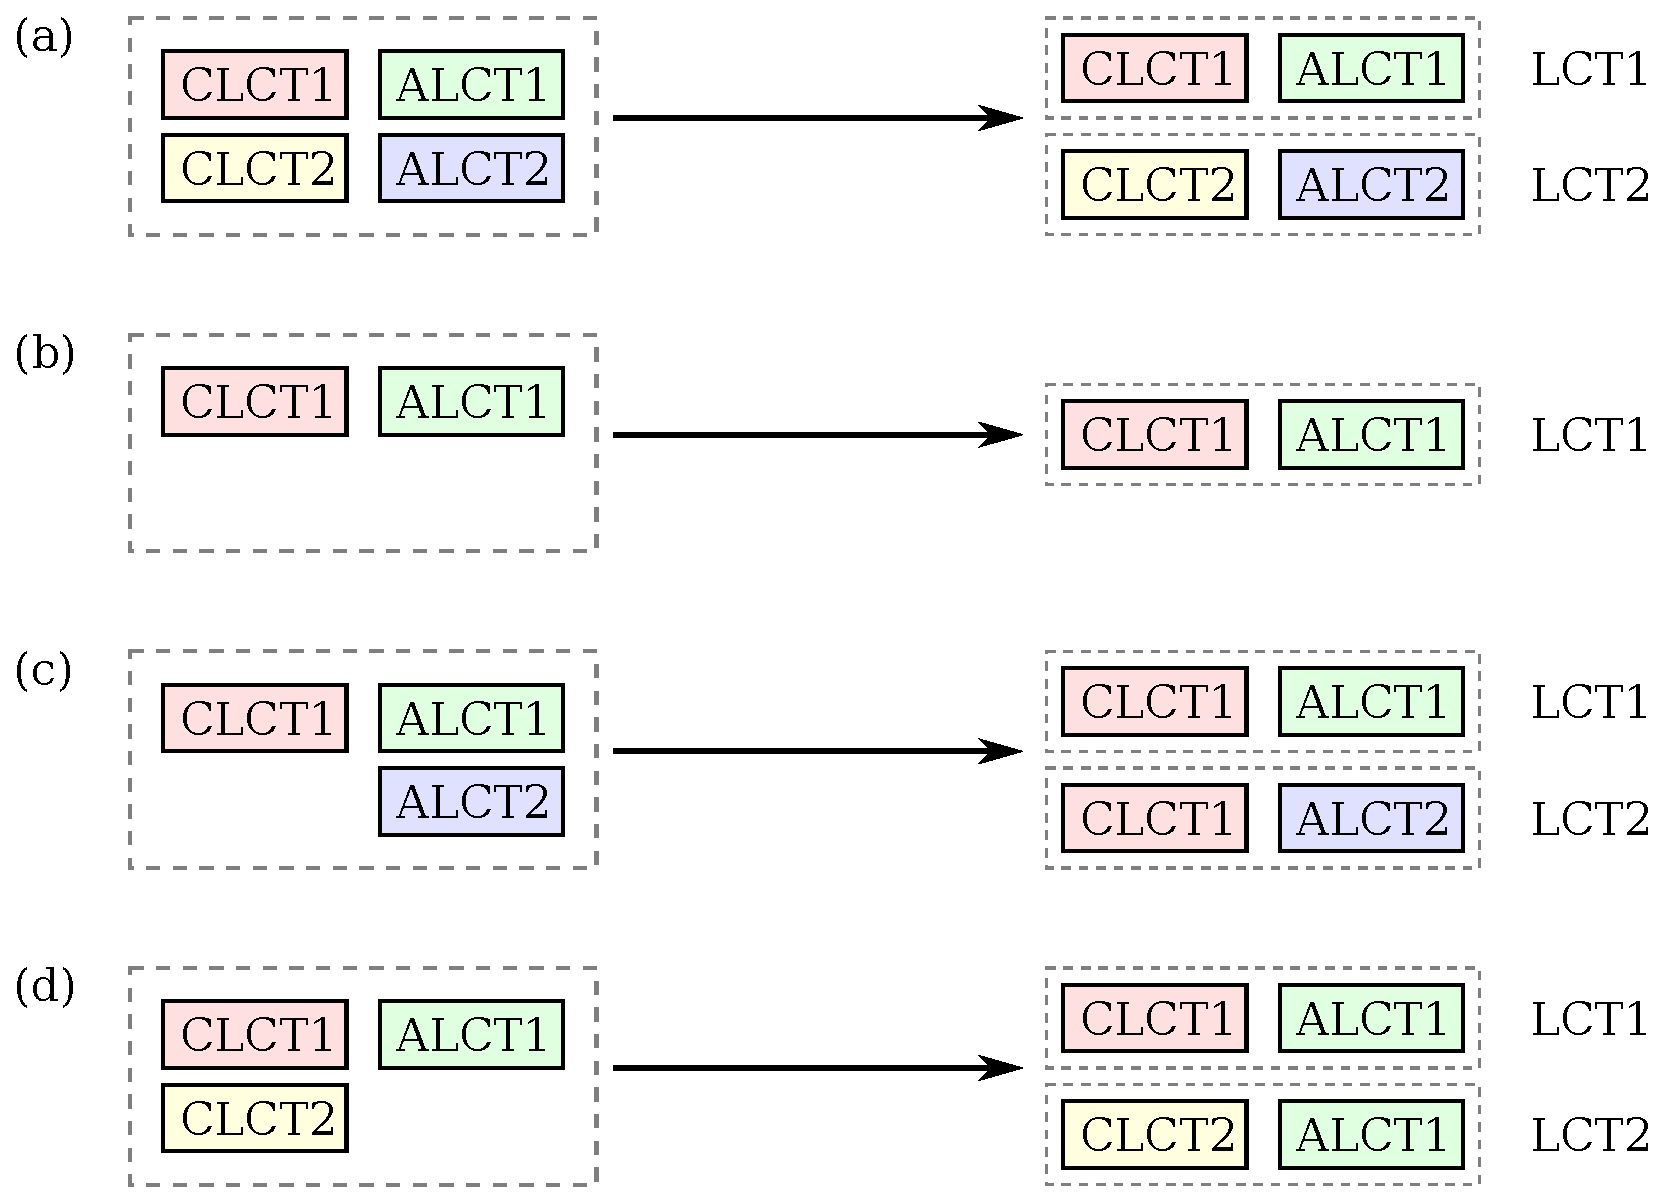
\includegraphics[width=0.7\linewidth]{figures/clct_alct_corr.pdf}
                \caption{Construction of LCTs.}
                \label{fig:clct_alct_corr}
        \end{center}
\end{figure}

But when, for example, there is only one valid CLCT and two valid ALCTs, we make the second valid CLCT from the first, analogously, when there are two valid CLCTs and only one valid ALCT (see bottom two examples on Fig.~\ref{fig:clct_alct_corr}).